\documentclass[11pt,headings=small]{scrartcl}
\usepackage{boschsensortec}
\usepackage{subcaption}
\usepackage{titlesec}
\usepackage{graphicx}
\usepackage{sidecap}
\usepackage{caption}
\usepackage{enumitem}
\usepackage{usnomencl}


\setcounter{secnumdepth}{4}
\titleformat{\paragraph}
{\normalfont\normalsize\bfseries}{\theparagraph}{1em}{}
\titlespacing*{\paragraph}
{0pt}{3.25ex plus 1ex minus .2ex}{1.5ex plus .2ex}

\RBtitleA{Bosch Sensortec}
\RBtitleB{COINES}
\RBtitleC{COmmunication for INertial and Environmental Sensors}

\BSTdocumentNumber{BST-DHW-AN013}
\BSTdocumentRevision{1.8}
\BSTdocumentReleaseDate{November 2023}
\BSTtechnicalReferenceCodes{n.a.}
\BSTdocumentType{User Manual}

%%-----------------------------------------------------------------------------
% Document begins here
%%-----------------------------------------------------------------------------
\begin{document}

\bstfirstpage
\tableofcontents
\newpage

\begin{Nomencl}[5em]
	\NomGroup{{\Large Acronyms and abbreviations }}
	\item[APP2.0] Application Board 2.0
	\item[APP3.x] Application Board 3.0 and Application Board 3.1
	\item[BLE] Bluetooth Low Energy
	\item[COINES] Communication with Inertial and Environmental Sensors
	\item[DFU] Device Firmware Upgrade
	\item[DTR] Data Terminal Ready
	\item[MCU] Microcontroller Unit
	\item[MEMS] Micro-Electro-Mechanical Systems
	\item[SDK] Software Development Kit
	\item[USB] Universal Serial Bus
\end{Nomencl}

\newpage

\section{Introduction}

Bosch Sensortec offers a toolkit for evaluation of it's sensor products.The toolkit consists of 3 elements:

\begin{enumerate}
	
	\item \textbf{Engineering board}: \href{https://www.bosch-sensortec.com/bst/support_tools/application_boards/overview_application_boards}{Application Board} named APP2.0 and APP3.x in this document, serves as interface translator from the sensor interface (I\textsuperscript{2}C or SPI) to a USB interface, allowing PC software to communicate with the sensor on the shuttle board. \href{https://store.arduino.cc/products/nicla-sense-me}{Nicla Sense ME} board combines four state-of-the-art sensors from Bosch Sensortec (BHI260AP, BMP390, BMM150 and BME688) in the Arduino ecosystem.
	
	\begin{figure}[H]
		\begin{center}
			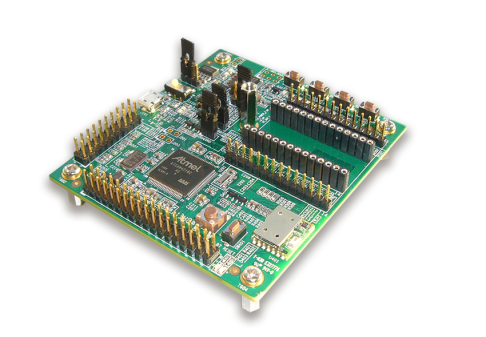
\includegraphics[width=0.50\textwidth]{coinesAPI_images/APP20-APP20.png}
			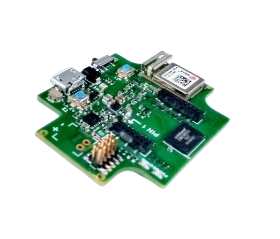
\includegraphics[width=0.40\textwidth]{coinesAPI_images/APP30.png}
			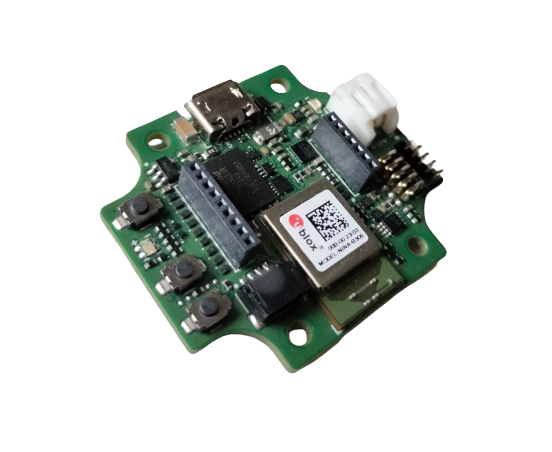
\includegraphics[width=0.40\textwidth]{coinesAPI_images/APP31.png}
			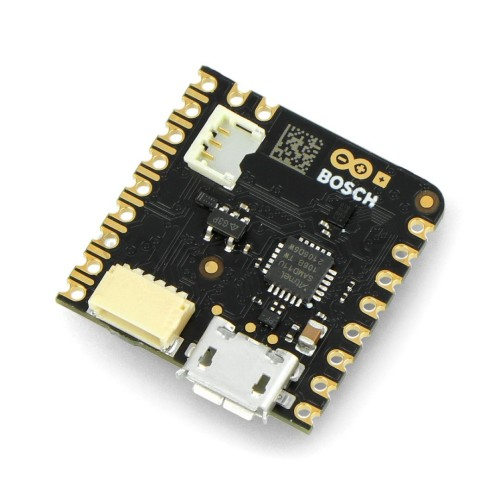
\includegraphics[width=0.40\textwidth]{coinesAPI_images/NiclaSenseME.jpg}
			\caption{Application Board 2.0/3.0/3.1/Nicla Sense ME}
		\end{center}
	\end{figure}

	\item \textbf{Sensor Shuttle board}: A sensor specific shuttle board also known as breakout board is a PCB with the sensor mounted on it. The shuttle board allows easy access to the sensor pins via a simple socket and can be directly plugged into the Bosch Sensortec’s Application boards. APP3.x shuttle boards also known as mini shuttle boards has smaller form factor when compared with APP2.0 shuttle board.
	
	\begin{figure}[H]
		\begin{center}
			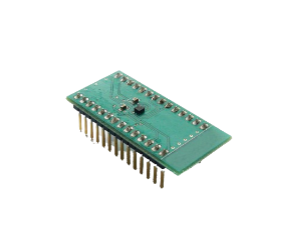
\includegraphics[width=0.35\textwidth]{coinesAPI_images/BMA222E_1.png}
			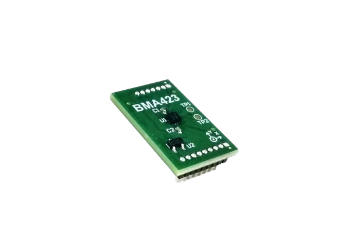
\includegraphics[width=0.45\textwidth]{coinesAPI_images/BMA423.png}
			\caption{APP2.0/3.x sensor shuttle board}
		\end{center}
	\end{figure}

	\item \textbf{COINES}: COINES provides a low-level interface for communication with Bosch Sensortec's Engineering boards enabling access to their MEMS sensors through sample applications and SensorAPI. For detailed description, refer to sections below.
\end{enumerate}

\newpage

\section{Introduction to COINES}

COINES ("\textbf{CO}mmunication with \textbf{IN}ertial and \textbf{E}nvironmental \textbf{S}ensors") is an SDK (Software Development Kit), implemented in C as a programming language that provides a low-level interface to Bosch Sensortec's Engineering Boards. The user can access Bosch Sensortec's MEMS sensors through this C interface. COINES can be used with the SensorAPI of the sensor which is available at \url{https://github.com/BoschSensortec}. The user can modify, compile and run the sample applications in COINES SDK and SensorAPI.


The full working environment consists of:
\begin{itemize}
	\item A Bosch Sensortec MEMS sensor on a shuttle board mounted on the socket of Bosch Sensortec's Application board APP2.0/APP3.x
	\item Windows, Linux or Mac PC to which the Engineering Board is connected via USB or BLE.
	\item The release of the COINES software is available at \url{https://www.bosch-sensortec.com/software-tools/tools/coines/}
	\item C compiler is also required (for details, see sections below)
\end{itemize}

\section{COINES usage}
The following diagram represents COINES usage.
\begin{figure}[H]
	\begin{center}
		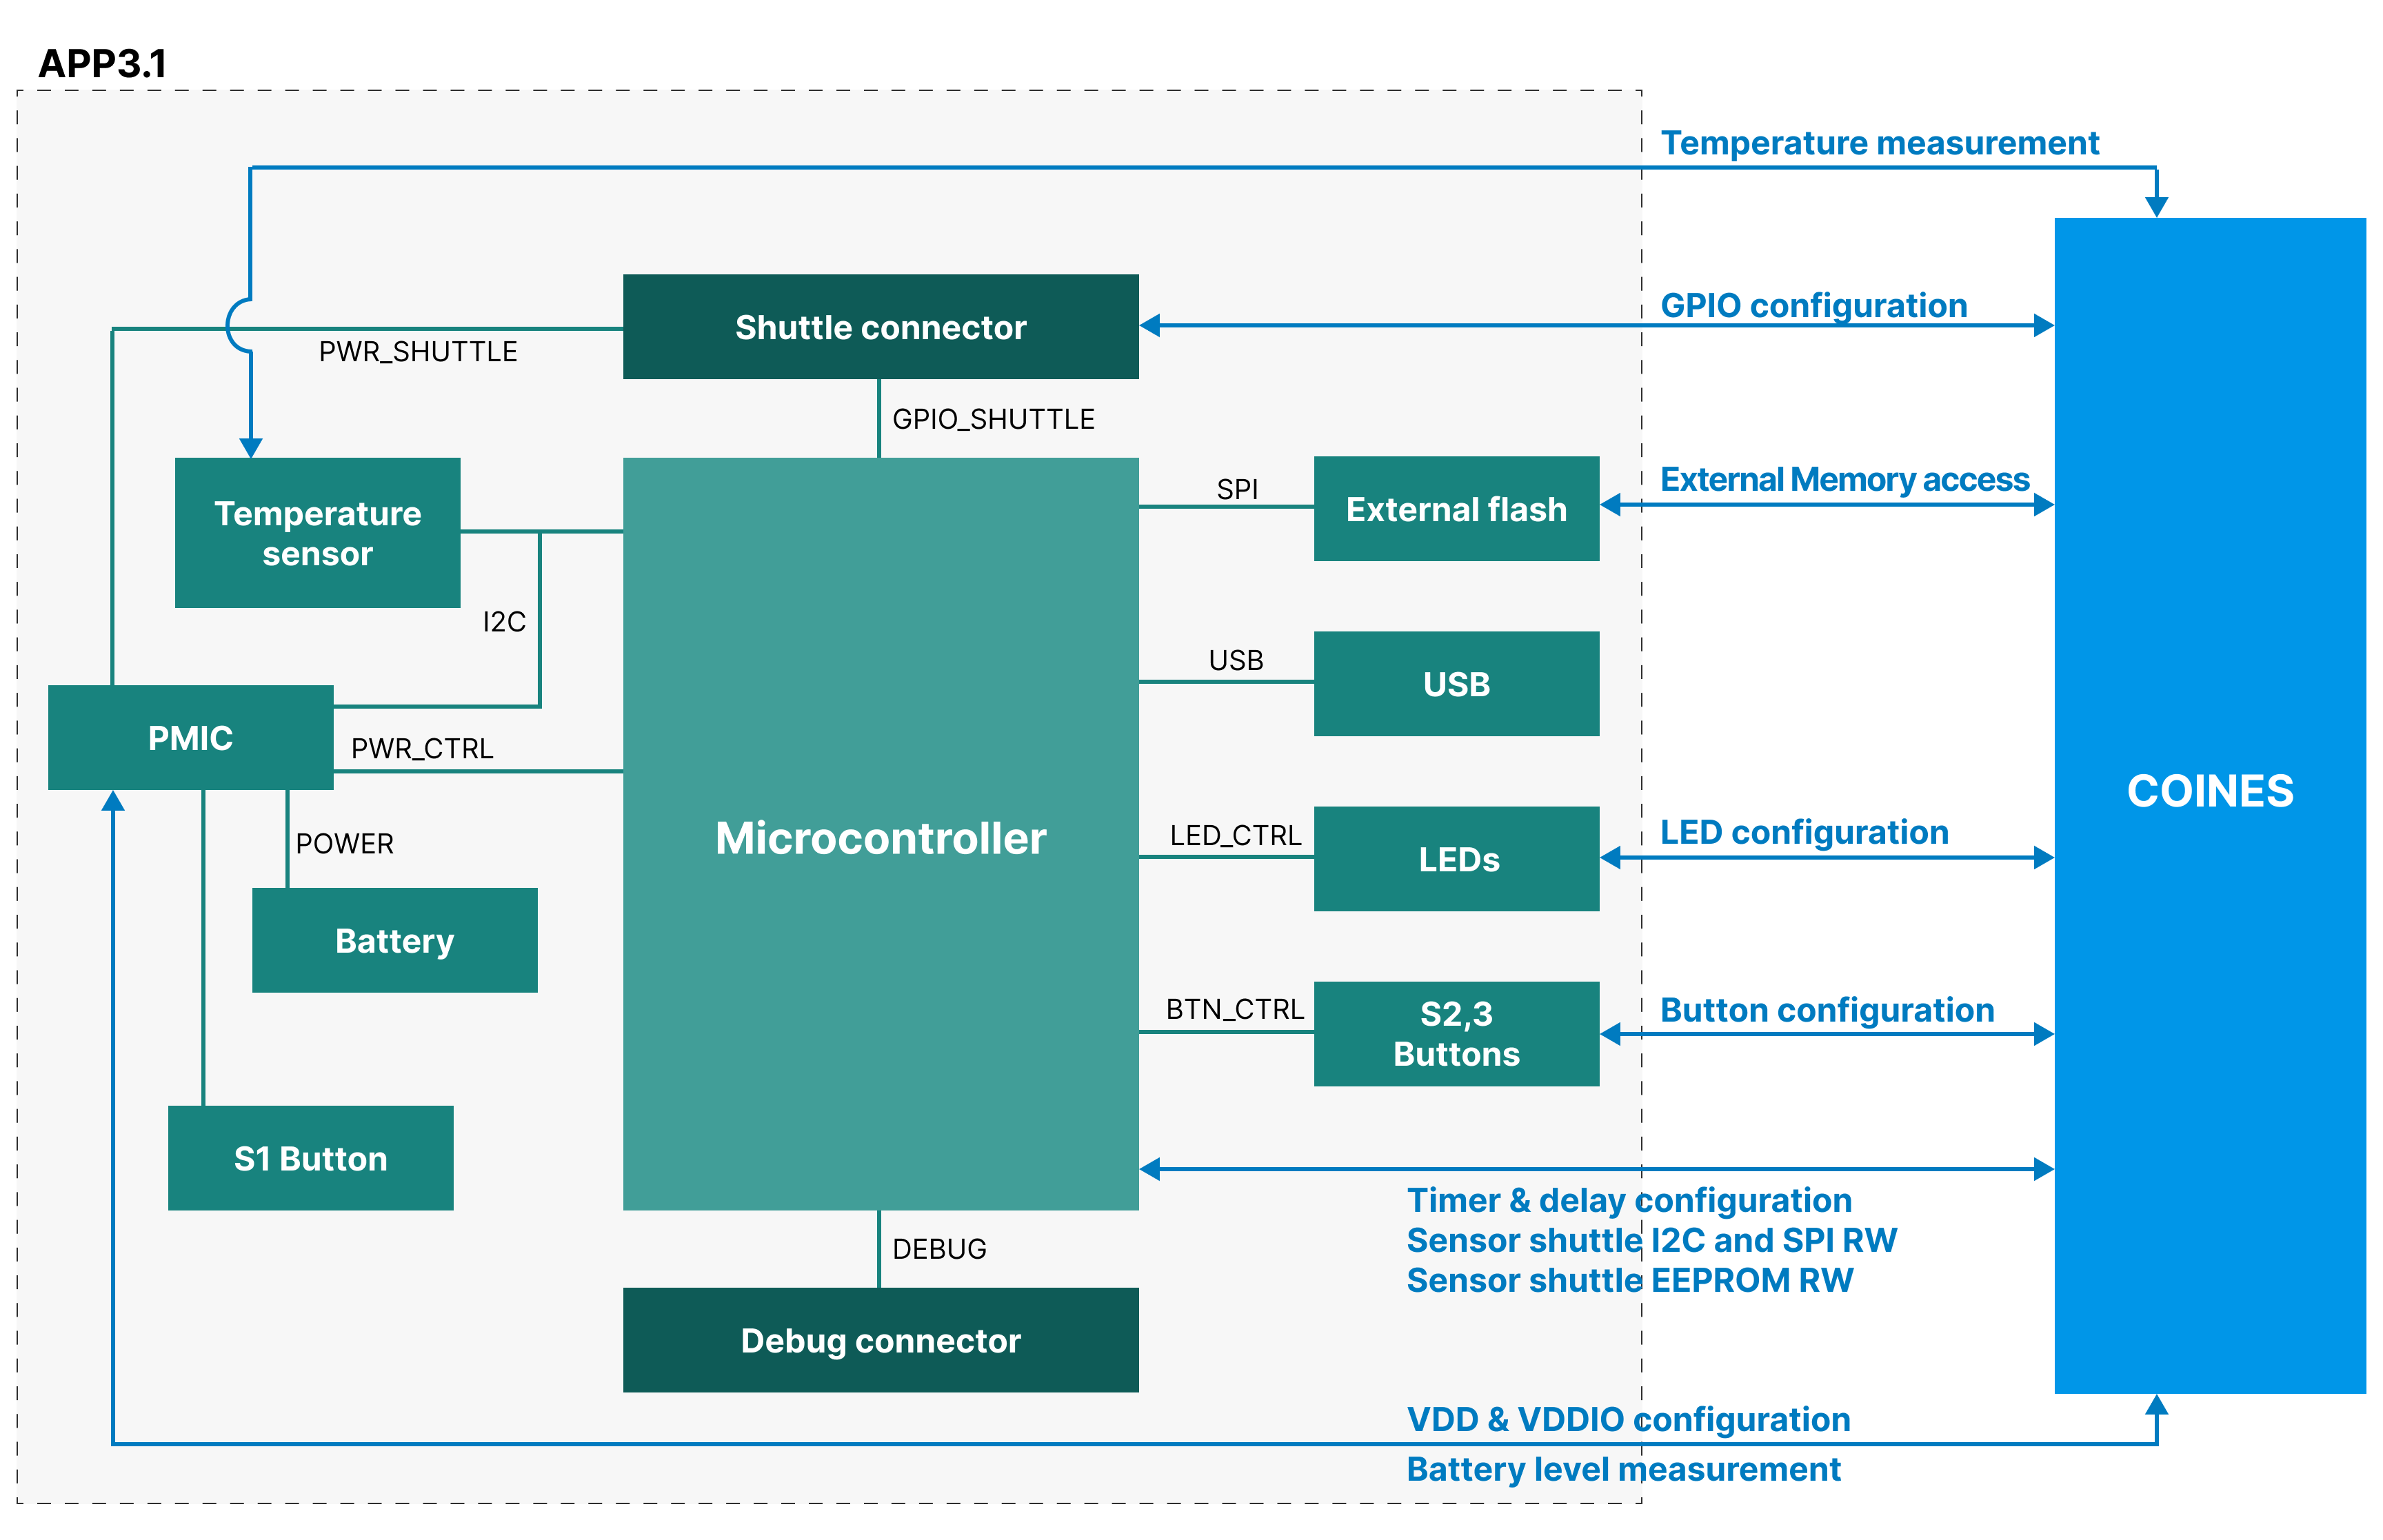
\includegraphics[width=1.1\textwidth]{coinesAPI_images/COINES_block_diagram.png}
		\caption{COINES usage with APP3.1}
	\end{center}
\end{figure}

\section{Installation}

COINES should be usable on any recent PC or laptop system which has at least a performance as an “office PC”. The hardware should provide a USB interface.

COINES runs on recent versions of Windows, Linux and Mac Operating systems.

\subsection{Installation (Windows)}

\subsubsection{System requirements}
The supported OS versions are Windows 10 and 11.

\subsubsection{Installation of COINES}
The steps below need to be followed in order to install COINES SDK:
\begin{enumerate}
	\item Download the latest version of COINES from \href{https://www.bosch-sensortec.com/software-tools/tools/coines/}{Bosch Sensortec website}
	\item Run the Installer
	\item Accept the End User License Agreement and click Next
	\begin{figure}[H]
		\begin{center}
			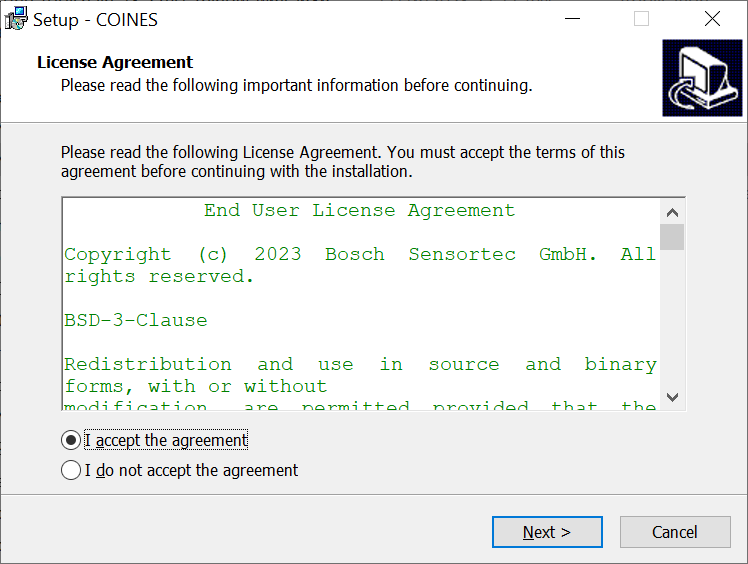
\includegraphics[width=0.7\textwidth]{coinesAPI_images/Windows_installation_user_agreement.png}
			\caption{Windows installer end user agreement dialog}
		\end{center}
	\end{figure}
	\item Click Install to start Installation
	\begin{figure}[H]
		\begin{center}
			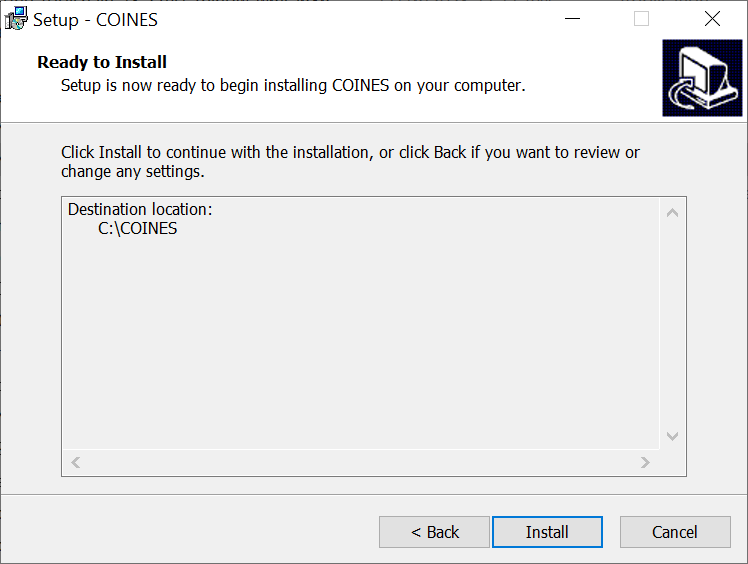
\includegraphics[width=0.7\textwidth]{coinesAPI_images/Windows_install_dialog.png}
			\caption{Windows install dialog}
		\end{center}
	\end{figure}
\end{enumerate}

\subsubsection{Installation of compiler environment}

COINES examples can be built using GNU C compiler (GCC). There are various distributions of GCC. TDM-GCC is easy to install and hence preferred for COINES. TDM GCC is based on MinGW GCC.

If you have already installed GCC (MinGW/Cygwin/MSYS2 GCC) and added to 'PATH' environmental variable, you can skip compiler installation.

The steps to install compiler environment are as follows:
\begin{enumerate}
	\item Download the TDM32/TDM64 bundle (\href{http://tdm-gcc.tdragon.net/}{link}). \textbf{Use TDM32 bundle if your Windows OS is 32-bit and TDM64 bundle if 64-bit.}
	\item Start the Installer. Ensure that the option Check for updated files on the TDM GCC server is unchecked. Click Create and proceed with the installation
	\item If you intend to do run the COINES example on Application Board's microcontroller, install the latest version of \href{https://developer.arm.com/downloads/-/arm-gnu-toolchain-downloads}{GNU Embedded Toolchain for ARM} for Windows. Make sure you have checked 'Add to PATH'.
\end{enumerate}


\begin{figure}[H]
	\begin{center}
		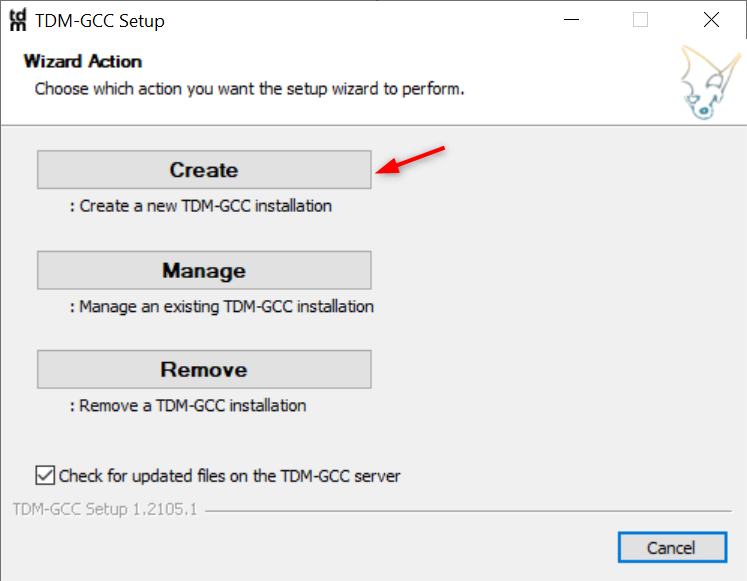
\includegraphics[width=0.7\textwidth]{coinesAPI_images/COINES_tdm-gcc-InstallationDialog.png}
	\end{center}
\end{figure}
\begin{figure}[H]
	\begin{center}
		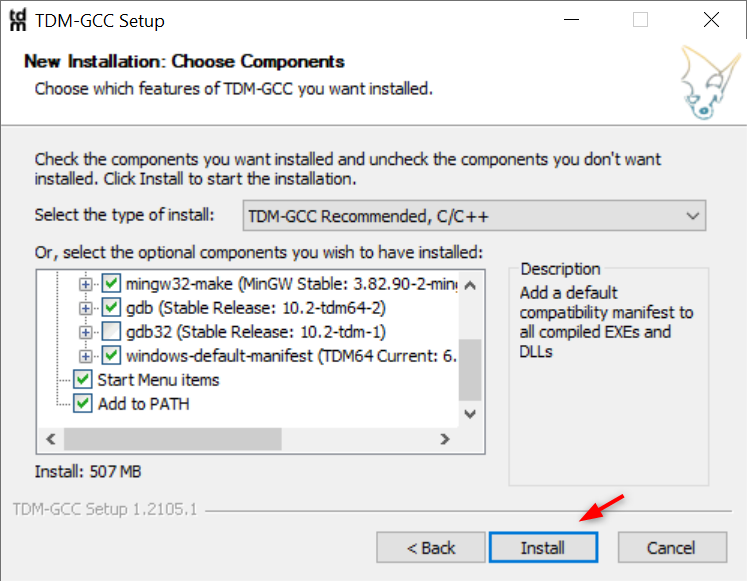
\includegraphics[width=0.7\textwidth]{coinesAPI_images/COINES_tdm-gcc-InstallationDialog_1.png}
		\caption{TDM-GCC installation dialog}
	\end{center}
\end{figure}

\begin{figure}[H]
	\begin{center}
		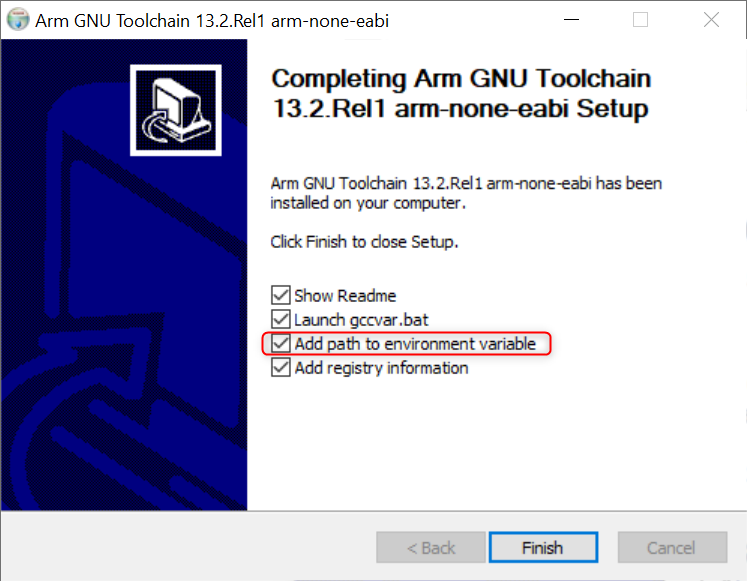
\includegraphics[width=0.7\textwidth]{coinesAPI_images/gnu_arm_toolchain_installation.png}
		\caption{GNU ARM Toolchain installation}
	\end{center}
\end{figure}


\newpage
\subsection{Installation (Linux/MacOS)}
  
\subsubsection{System requirements}

\begin{itemize}
	\item The supported Linux OS versions are Debian based - Ubuntu 18.04 and 22.04.
	\item  The supported macOS versions are MacOS Ventura 13.4.1 and 13.5.2.
\end{itemize} 

\subsubsection{Installation of COINES}
The steps below need to be followed in order to install COINES SDK:
\begin{enumerate}
	\item Download the installer.
	\item Use the command \texttt{cd} to go to the directory where the installer is located and make the installer executable:
	\begin{itemize}
		\item[\$] \texttt{chmod +x coines\_vX.Y.sh}
	\end{itemize}
	\item Ensure that you are connected to the Internet before running the installer, which is executed like this:
	\begin{itemize}
	\item[\$] \texttt{./coines\_vX.Y.sh}
	\end{itemize}	
	\item Accept the End User License agreement
	\begin{figure}[H]
		\begin{center}
			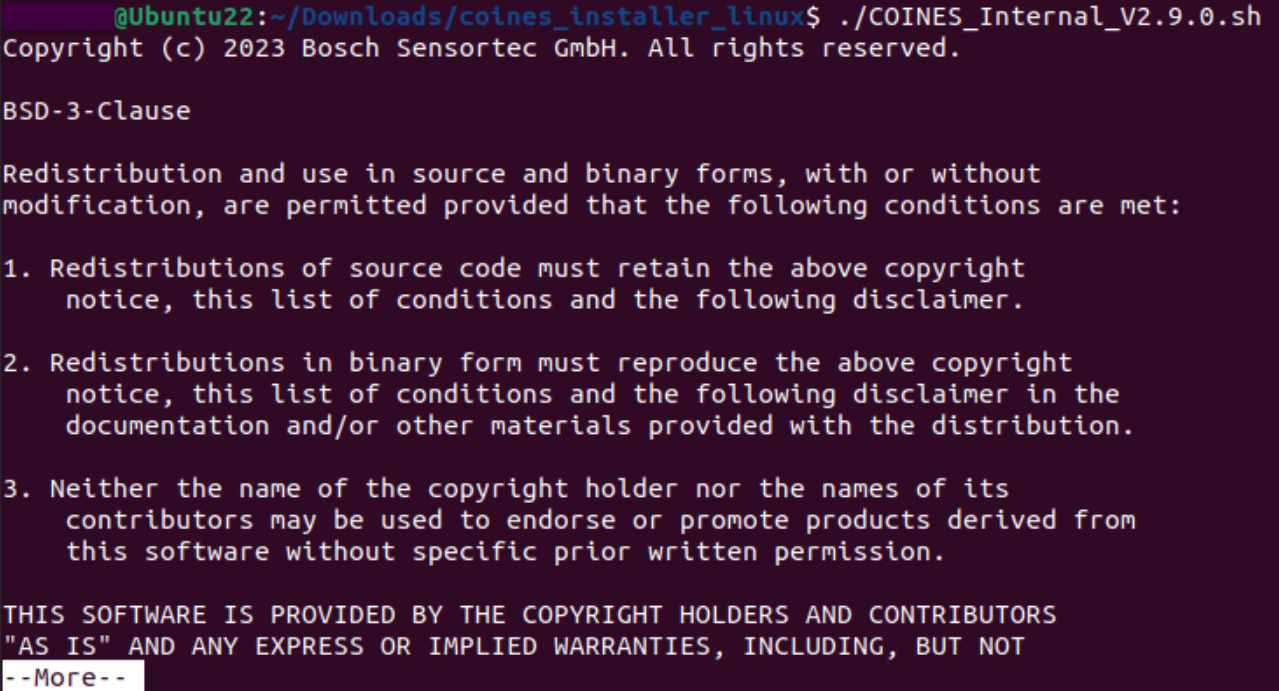
\includegraphics[width=0.7\textwidth]{coinesAPI_images/Linux_installation_user_agreement.png}
		\end{center}
	\end{figure}
	\begin{figure}[H]
		\begin{center}
			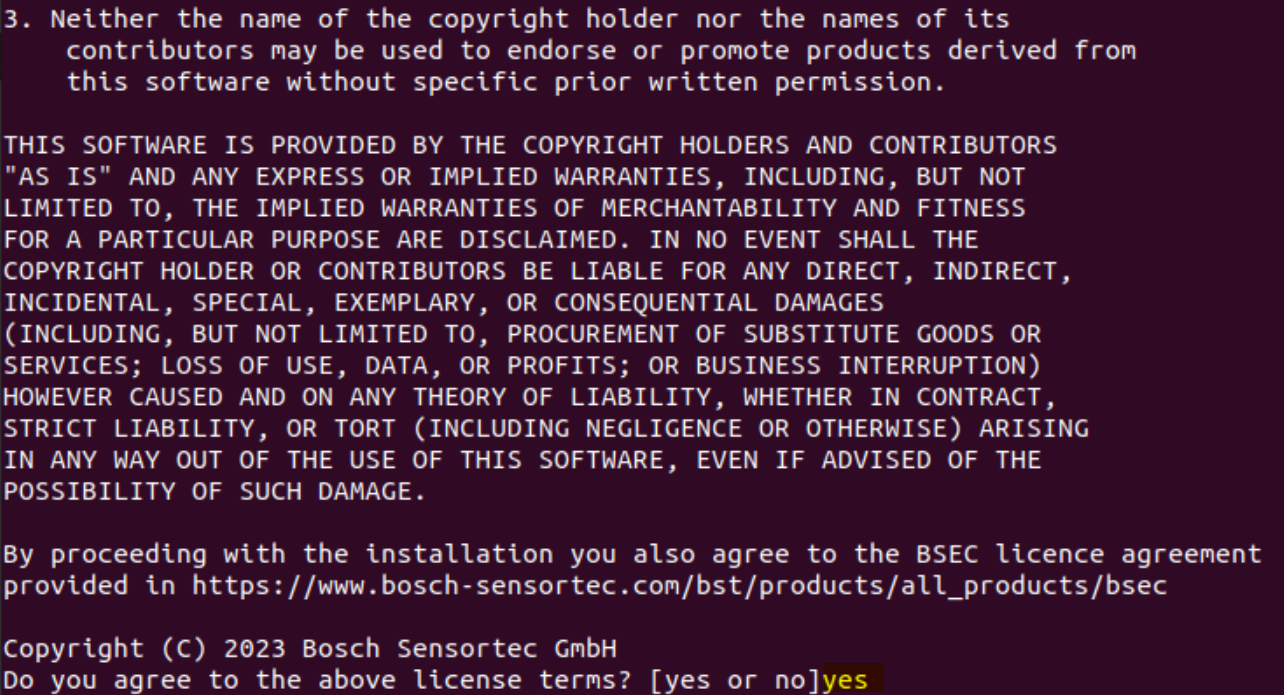
\includegraphics[width=0.7\textwidth]{coinesAPI_images/Linux_installation_user_agreement_1.png}
			\caption{Linux installer end user agreement}
		\end{center}
	\end{figure}
	\item The installer will prompt you if the required dependencies/packages are not installed. (This step requires root privileges.)
\end{enumerate}

\subsubsection{Installation of compiler environment}

On a Debian or Redhat based Linux distro, the installer prompts for installation of missing dependencies, \texttt{gcc}, \texttt{make} and \texttt{libusb-dev} packages.If due to some reason installation fails, the user can manually install the dependencies.
\begin{itemize}
\item Debian based distros - \texttt{gcc}, \texttt{make}, \texttt{libusb-1.0-0-dev}, \texttt{dfu-util} , \texttt{libdbus-1-dev}
\item Redhat based distros - \texttt{gcc}, \texttt{make}, \texttt{libusbx-devel}, \texttt{dfu-util}, \texttt{dbus-devel}
\item MacOS - 
\texttt{libusb}, \texttt{dfu-util}
\end{itemize}

If you intend to run the COINES example on Application Board's microcontroller, download the latest version of \href{https://developer.arm.com/downloads/-/arm-gnu-toolchain-downloads}{GNU Embedded Toolchain for ARM} for Linux and extract the package. Add the compiler to PATH variable by editing \texttt{\$HOME/.bashrc} or similar file like \texttt{/etc/profile or /etc/environment}.

\section{Using COINES to access the sensor on Engineering Board} \label{coines}

\subsection{Running examples on the MCU of the Application board}\label{ExampleOnMCU}
\subsubsection{Working principle}
The COINES SDK can be cross-compiled on PC side and downloaded into the memory of the Application board and executed there. The user can choose to download the created binary into the flash memory or into the RAM (if the binary is within the RAM memory capacity e.g., APP3.x's RAM is 256 KB).

Downloading COINES SDK example to APP3.x Flash memory will overwrite default firmware. To update the firmware again, refer to section \ref{firmwareUpdate}.

In this configuration, the COINES layer provides a simple abstraction on top of the MCU BSP (i.e. board level support layer of the microcontroller). Any \texttt{printf} command will now not output to the console, but rather to the USB connection, which appears as virtual COM port on PC side.

This mode facilitates the execution of many time-critical operations on the sensor, such as fast reading of FIFO content at high data rates.

\begin{figure}[H]
	\begin{center}
		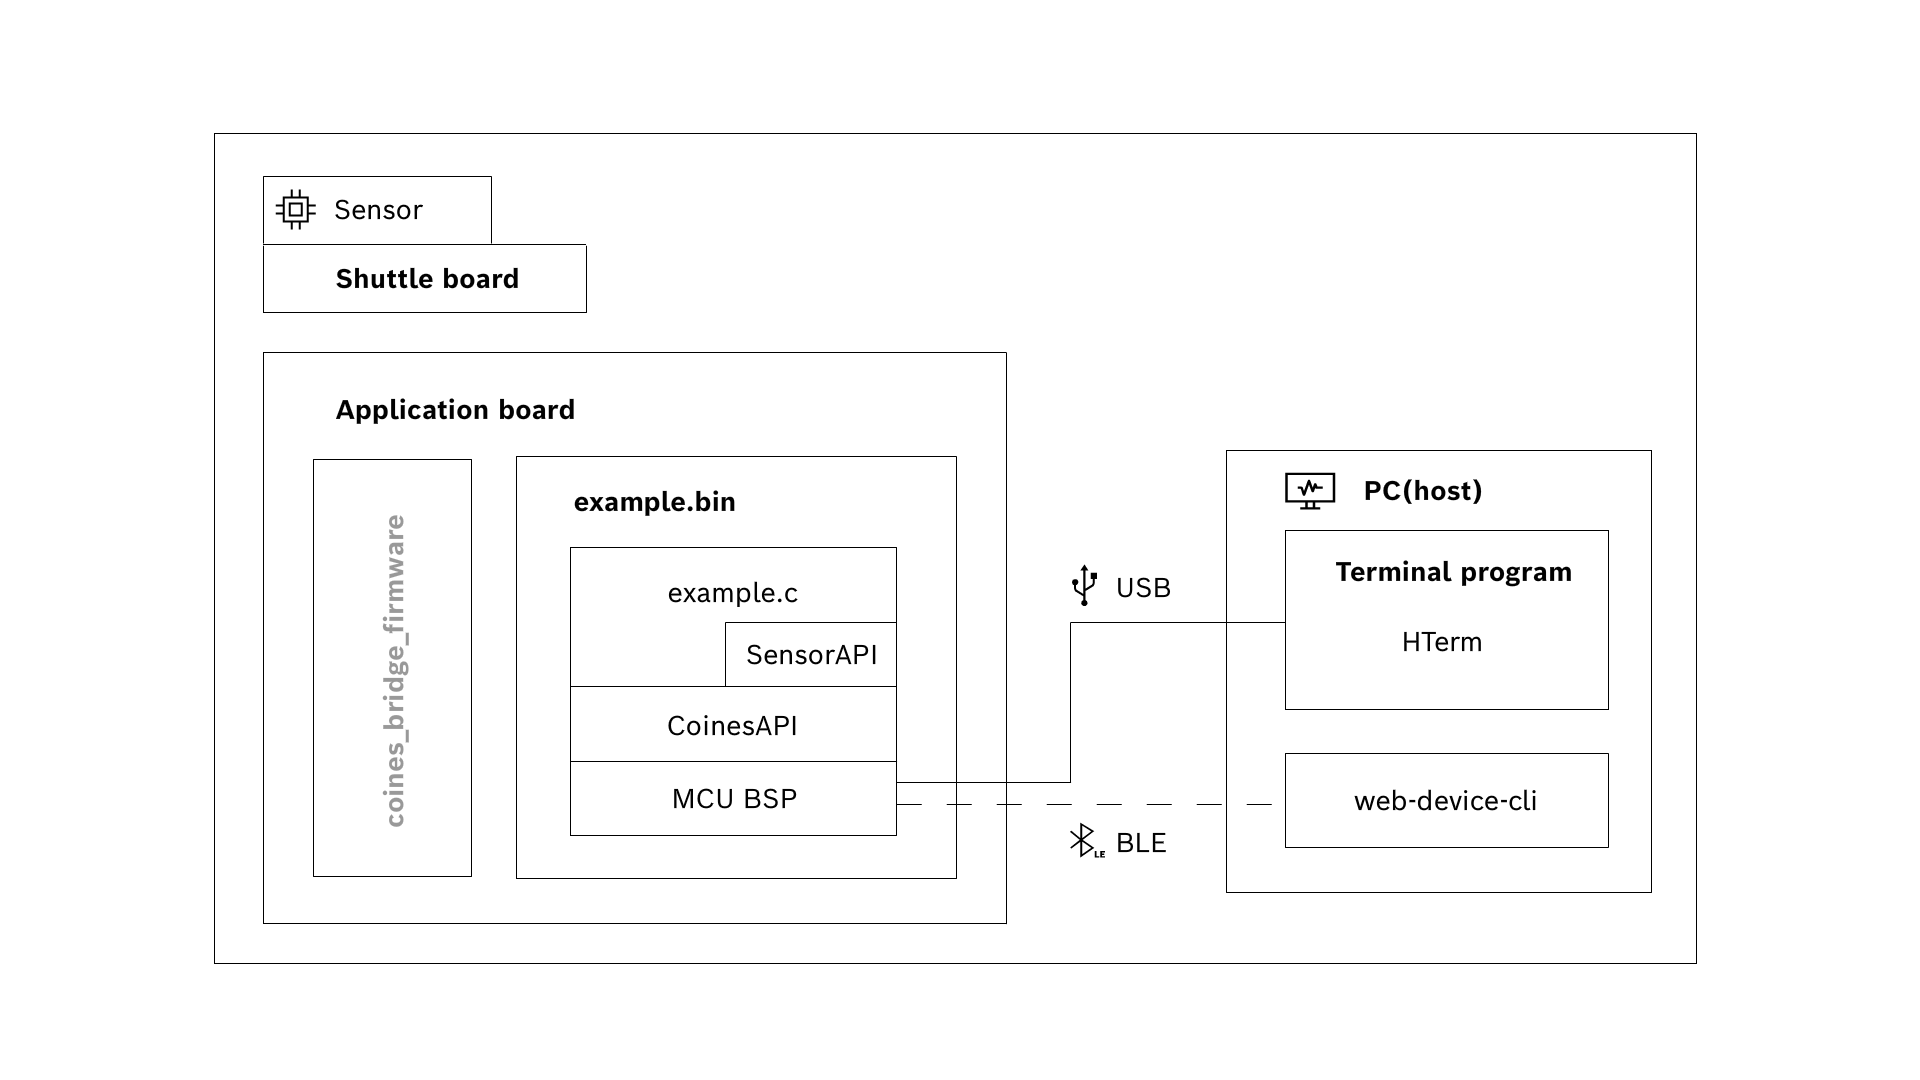
\includegraphics[width=0.9\textwidth]{coinesAPI_images/COINES_workingPrinciple_runOnMCU.png}
		\caption{Working principle: Running example on the MCU of the Application board}
	\end{center}
\end{figure}

\subsubsection{Getting started}
To get started with example execution, follow these steps:
\begin{enumerate}
	\item Make sure that \href{https://developer.arm.com/downloads/-/arm-gnu-toolchain-downloads}{GNU Embedded Toolchain for ARM} is installed on your PC and added to environmental variable \texttt{PATH}.
	\item Connect the Application board via USB, with the sensor shuttle board mounted.
	\item Open the command prompt or the terminal.
	\item Use the command \texttt{cd} to go to the directory where the example that is to be built is located.
\end{enumerate}

\subsubsection{Interfacing via BLE}
The procedure to interface via BLE involves these steps:
\begin{enumerate}
	\item Open the script to be executed (in case of SensorAPI - common.c file in the selected example folder) in your IDE
	\item Change COINES\_COMM\_INTF\_USB  to COINES\_COMM\_INTF\_BLE
	\item Change all print statments
	\begin{verbatim}
	printf(...) to fprintf(bt_w,...)
	\end{verbatim}
	\item Now follow the steps from 1 - 4 in the above section
\end{enumerate}

\subsubsection{Cross compiling}
To compile and download an example to Engineering Board's microcontroller, type any of the build commands below based on available Engineering board type and target memory location. Use '\texttt{mingw32-make}' (TDM-GCC/MinGW) or '\texttt{make}' (Linux/Cygwin/MSYS2/MacOS) for compilation.
\begin{table}[H]
	\centering
	\resizebox{\textwidth}{!}{
	\begin{tabular}{|l|l|}
		\hline
		Download example to APP2.0 MCU RAM & \texttt{mingw32-make LOCATION=RAM TARGET=MCU\_APP20 download} \\ \hline
		Download example to APP2.0 MCU FLASH & \texttt{mingw32-make LOCATION=FLASH TARGET=MCU\_APP20 download} \\ \hline
		Download example to APP3.0 MCU RAM & \texttt{mingw32-make LOCATION=RAM TARGET=MCU\_APP30 download} \\ \hline
		Download example to APP3.0 MCU FLASH & \texttt{mingw32-make LOCATION=FLASH TARGET=MCU\_APP30 download} \\ \hline
		Download example to APP3.1 MCU RAM & \texttt{mingw32-make LOCATION=RAM TARGET=MCU\_APP31 download} \\ \hline
		Download example to APP3.1 MCU FLASH & \texttt{mingw32-make LOCATION=FLASH TARGET=MCU\_APP31 download} \\ \hline
		Run an example already residing in APP2.0 Flash memory & \texttt{mingw32-make run} \\ \hline 
	\end{tabular}}
\end{table}
Note: Nicla board programs can only be executed as PC target at this moment.

\subsubsection{Viewing the results}
The ways to view the execution results are outlined as follows:
\begin{enumerate}
	\item Use a Serial Terminal application to view output.
	\begin{itemize}
		\item Windows - PuTTY, HTerm,etc.,
		\item Linux - \texttt{cat} command. Eg: \texttt{cat /dev/ttyACM0}
		\item macOS - \texttt{screen} command. Eg: \texttt{screen /dev/tty.usbmodem9F31}
	\end{itemize}
	Note: The binary on the MCU will be executed once the serial port is opened. The port must be opened including DTR signal set, otherwise the binary will not be executed. Some terminal programs such as HTerm allow explicit setting of the DTR signal.
	\item For bluetooth communication, connect the Application board to another power source and keep it within the BLE range. And use any of the below tools to view the output.
	\begin{itemize}
		\item Android app - \href{https://play.google.com/store/apps/details?id=de.kai_morich.serial_bluetooth_terminal}{Serial Bluetooth terminal}
		\item Website - \href{https://wiki.makerdiary.com/web-device-cli/}{Web Device CLI}
		\item Python script - \path{\tools\ble-nus-term\ble-nus-term.py}
	\end{itemize}
\end{enumerate}

\subsubsection{Data logging}
The user can use any serial terminal program to access and store the data provided via virtual COM port e.g HTerm has "Save output" option to store log.

\subsection{Running examples on PC side}
\subsubsection{Working principle}
When compiling the COINES SDK for PC side, the COINES layer provides an abstraction of the embedded environment on the host side. COINES library provides read and write functions for I\textsuperscript{2}C and SPI on PC side. These functions receive the arguments of the user input (i.e. what register address to read from) and tunnel them through the USB connection to the Application Board, where they are fed into the embedded I\textsuperscript{2}C and SPI functions and are executed to access the sensor. Any result or response from those functions is tunneled back to the PC side and provided to the example application.

This approach allows easy and flexible programming and offers the possibility to integrate the example code into other applications or add advanced logging options. The drawback is that in this mode the code is not executed in real time, as it runs on a multi-tasking operating system. To overcome this drawback, the examples can also be run on the MCU side (see section \ref{ExampleOnMCU}).

\begin{figure}[H]
	\begin{center}
		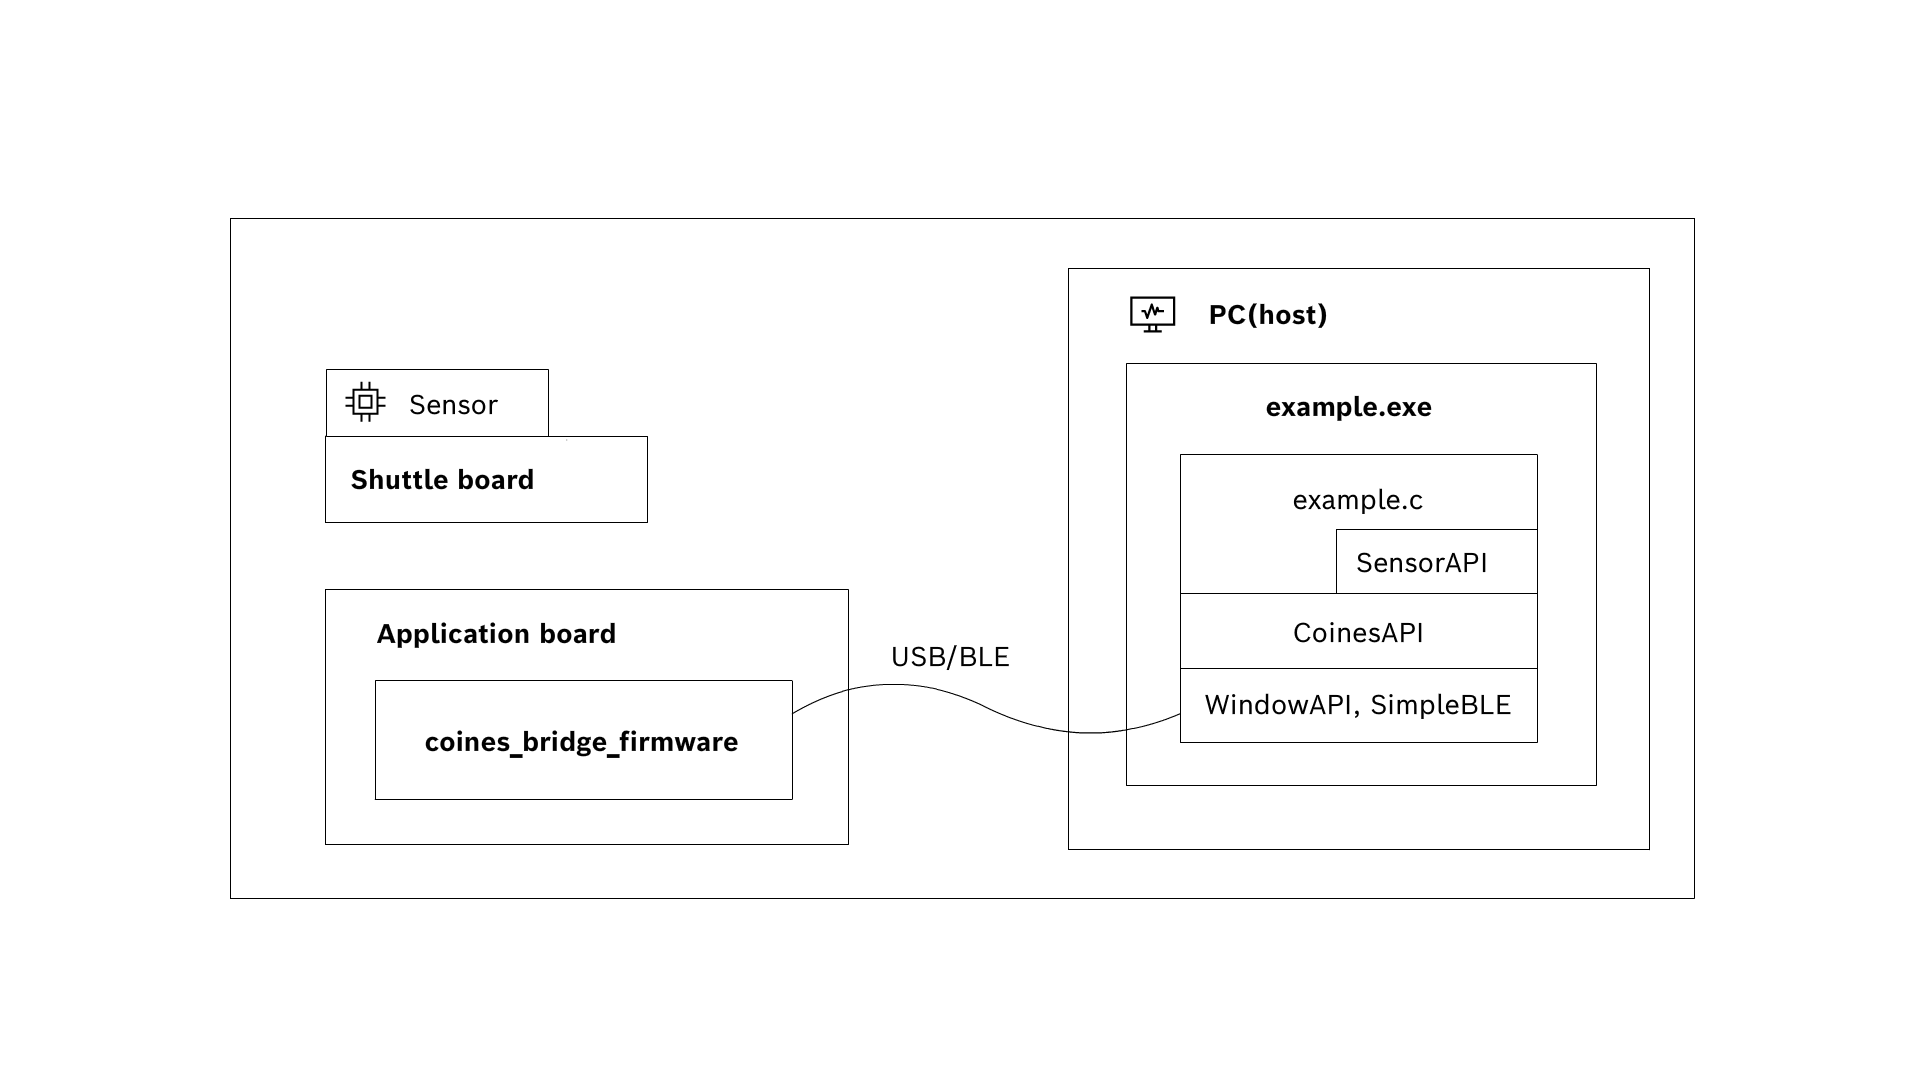
\includegraphics[width=0.9\textwidth]{coinesAPI_images/COINES_workingPrinciple_runOnPC.png}
		\caption{Working principle: Running example on PC side}
	\end{center}
\end{figure}

\subsubsection{PC side implementation}
This setup has the challenge of lacking the real-time capabilities known from a pure microcontroller environment. To overcome this, the coinesAPI offers streaming functions, which allow the user to schedule data readout directly on the microcontroller, either based on a data interrupt coming from the sensors or based on the timer of the microcontroller. The scheduler waits for the configured interrupt (sensor interrupt or timer interrupt) and reads out areas of the register map, which can be configured by the user.

As an example, the user could choose to read out the 6 bytes from the register map of a certain inertial sensor, containing the sensor data of three axis (2 bytes per axis). If the user would configure e.g a readout once per milliseconds, the result would be a data stream of three-axis sensor data at a rate of 1 kHz.

\subsubsection{Getting started}
To get started with example execution, follow these steps:
\begin{enumerate}
\item Connect the Application board via USB, with the sensor shuttle board mounted.
\item Refer to section \ref{firmwareUpdate} and update the Coines Bridge firmware to the board.
\item Open the command prompt or the terminal.
\item Use the command \texttt{cd} to go to the directory where the example that is to be built is located.
\end{enumerate}
Note: Some examples may not compile for both PC and MCU target. Please refer to the example documentation or simply the example name (e.g. examples that can only be compiled for the PC are named with a following '\_pc').

\subsubsection{Interfacing via BLE}
The procedure to interface via BLE involves these steps:
\begin{enumerate}
	\item Open the script to be executed (in case of SensorAPI - common.c file in the selected example folder) in your IDE
	\item Change COINES\_COMM\_INTF\_USB  to COINES\_COMM\_INTF\_BLE
	\item Now follow the steps from 1 - 4 in the above section
\end{enumerate}

\subsubsection{Compiling}
To run an example in PC side, execute below command "mingw32-make TARGET=PC". Use '\texttt{mingw32-make}' (TDM-GCC/MinGW) or '\texttt{make}' (Linux/Cygwin/MSYS2/MacOS) for compilation.

\subsubsection{Viewing the results}
Running the output executable in the command prompt of the PC will display the results. To view ouput via BLE, connect the Application board to another power source and keep it within the BLE range and run the executable in the PC.

\subsubsection{Data logging}

The user can utilize the terminal's output redirection command to store the result of a command/executable in a file, as demonstrated below.
\begin{figure}[H]
	\begin{center}
		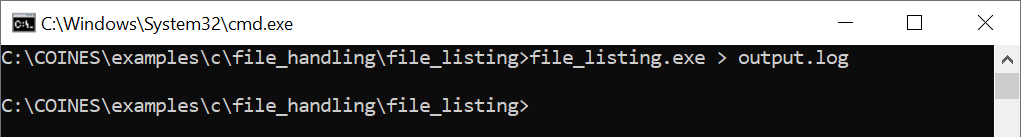
\includegraphics[width=0.9\textwidth]{coinesAPI_images/PC_data_logging.png}
	\end{center}
\end{figure}

\subsection{Project Cleanup}
The commands to clean build files are listed below:
\begin{itemize}
	\item \texttt{mingw32-make clean} - Use this command to remove the object files and other intermediate files created during the compilation process.
	\item \texttt{mingw32-make clean-all} - Use this command to remove all build artifacts, including the final executable or library, and start the build process from scratch
\end{itemize}

\section{Using COINESPY to access the sensor on Engineering Board}

\subsection{Introduction to \texttt{COINESPY} library}

The \texttt{COINESPY} library provides a Python interface for interacting with the Bosch Sensortec's Engineering Boards. 
\newline \newline The library offers the following range of functionalities:
\begin{itemize}
	\item Control VDD and VDDIO of sensor
	\item Configure SPI and I\textsuperscript{2}C bus parameters
	\item Read and write into registers of sensors from Bosch Sensortec via SPI and I\textsuperscript{2}C
	\item Read and write digital pins of the Application Board
\end{itemize}

\subsection{Installation}

The \texttt{COINESPY} module can be installed using pip:
\begin{lstlisting}
pip install coinespy
\end{lstlisting}
The module can be found on \url{https://pypi.org/project/coinespy/}.
It is highly recommended to test the following script \texttt{examples\textbackslash python\textbackslash coinespy\_test.py}  in the COINES installation or Refer to \ref{GettingBoardInfo} to check if the installation was successful.

\newpage
\section{Using Sensor API with COINES}
\subsection{SensorAPI}
Bosch Sensortec recommends using the SensorAPI in order to communicate with the sensors. The SensorAPI, an abstraction layer written in C makes it much more convenient for the user to access the register map of the sensor, in order to configure certain functionality and obtain certain information from it.

For making use of the SensorAPI, some function pointers must be set to the appropriate read/write functions of the selected bus on the system (either I\textsuperscript{2}C or SPI), as well as one function pointer to a system's function causing delays in milliseconds.

In order to execute C code using SensorAPI, the COINES API provides the mentioned read, write, delay functions. These functions are wrapper functions, embedding the actual SensorAPI payloads into a transport package, sending this via USB or BLE to the Engineering board, where the payload is translated into corresponding SPI or I\textsuperscript{2}C messages and sent to the sensor on the shuttle board.The mapping would look similar to the one below.

\begin{lstlisting}
#include "coines.h"
#include "bst_sensor.h"

struct bst_sensor_dev sensordev;
....
....
sensordev.intf = BST_SENSOR_I2C_INTF;  // SPI - BST_SENSOR_SPI_INTF
sensordev.read = coines_read_i2c;   // coines_read_spi
sensordev.write = coines_write_i2c; // coines_write_spi
sensordev.delay_ms = coines_delay_usec;

\end{lstlisting}

For the description of COINES functions used, refer to \ref{CoinesCFunctions}.

\subsection{Downloading Sensor API}
In order to download SensorAPI, the steps below need to be followed:
\begin{itemize}
	\item Download SensorAPI repo using Download zip option for selected sensors from boschsensortec github \url{https://github.com/BoschSensortec}.
	\item Unzip the downloaded SensorAPI repo to \path{\examples}.
	\item Rename the unzipped folder to sensor name e.g \path{\examples\bmi270} and change directory to an example folder to execute it.
\end{itemize}

\subsection{Running example on MCU side}
Here are the step-by-step instructions to run examples on MCU side:
\begin{itemize}
	\item Selected Platform: Windows
	\item Board: APP3.1
	\item Sensor shuttle: BMI270
	\item Example: \path{\examples\bmi270\bmi270_examples\accel_gyro}
\end{itemize}
\begin{enumerate}
	\item Connect the Application Board board via USB, with the sensor shuttle board mounted.
	\item Open the command prompt or the terminal.
	\item Use the command \texttt{cd} to go to the directory where the example that is to be built is located.
	\begin{figure}[H]
		\begin{center}
			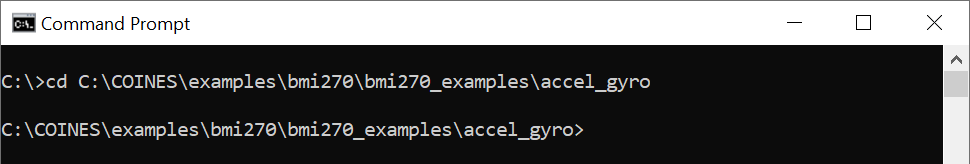
\includegraphics[width=0.9\textwidth]{coinesAPI_images/Mcu_example_cd.png}
		\end{center}
	\end{figure}
	\item Execute command "mingw32-make TARGET=MCU\_APP31 download"
	\begin{figure}[H]
		\begin{center}
			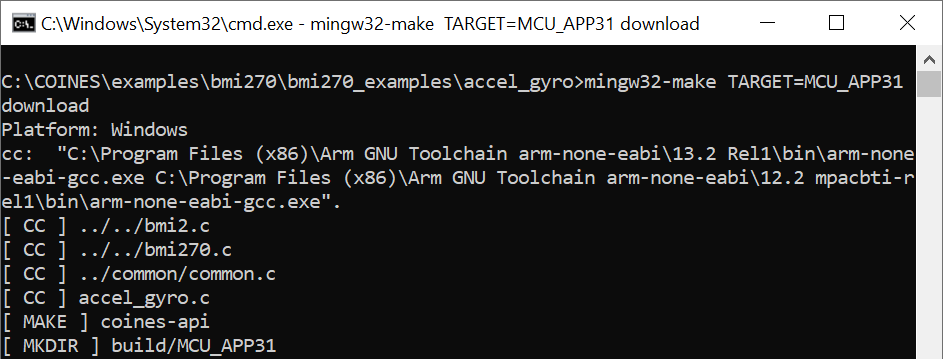
\includegraphics[width=0.9\textwidth]{coinesAPI_images/Mcu_example_compile.png}
		\end{center}
	\end{figure}
	\begin{figure}[H]
		\begin{center}
			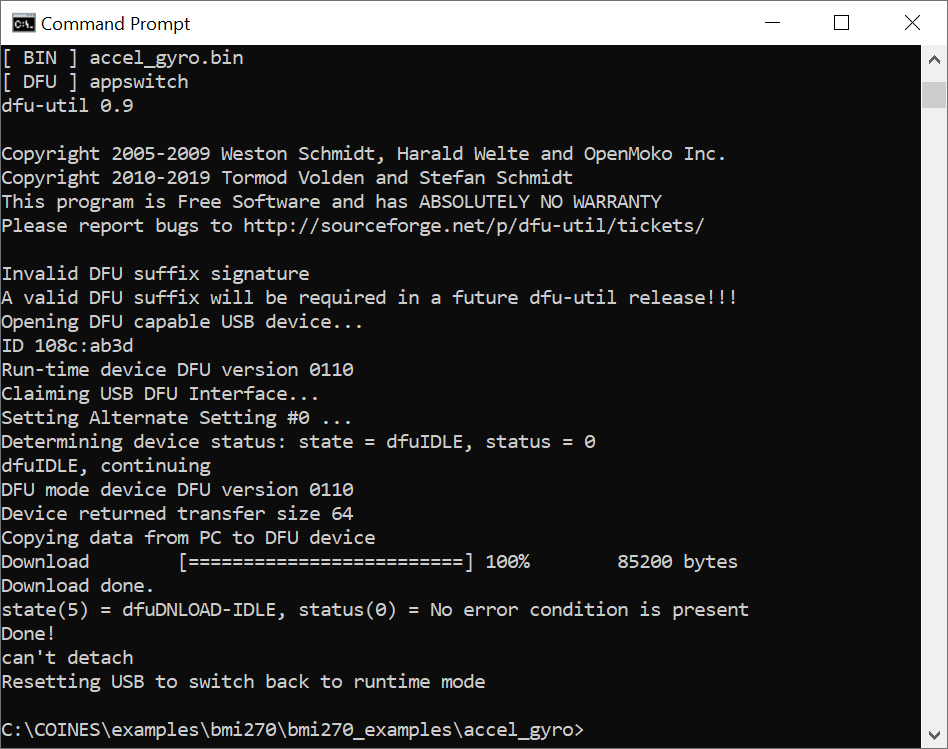
\includegraphics[width=0.9\textwidth]{coinesAPI_images/Mcu_example_download.png}
		\end{center}
	\end{figure}
	\item View the output in a serial terminal application like HTerm
	\begin{figure}[H]
		\begin{center}
			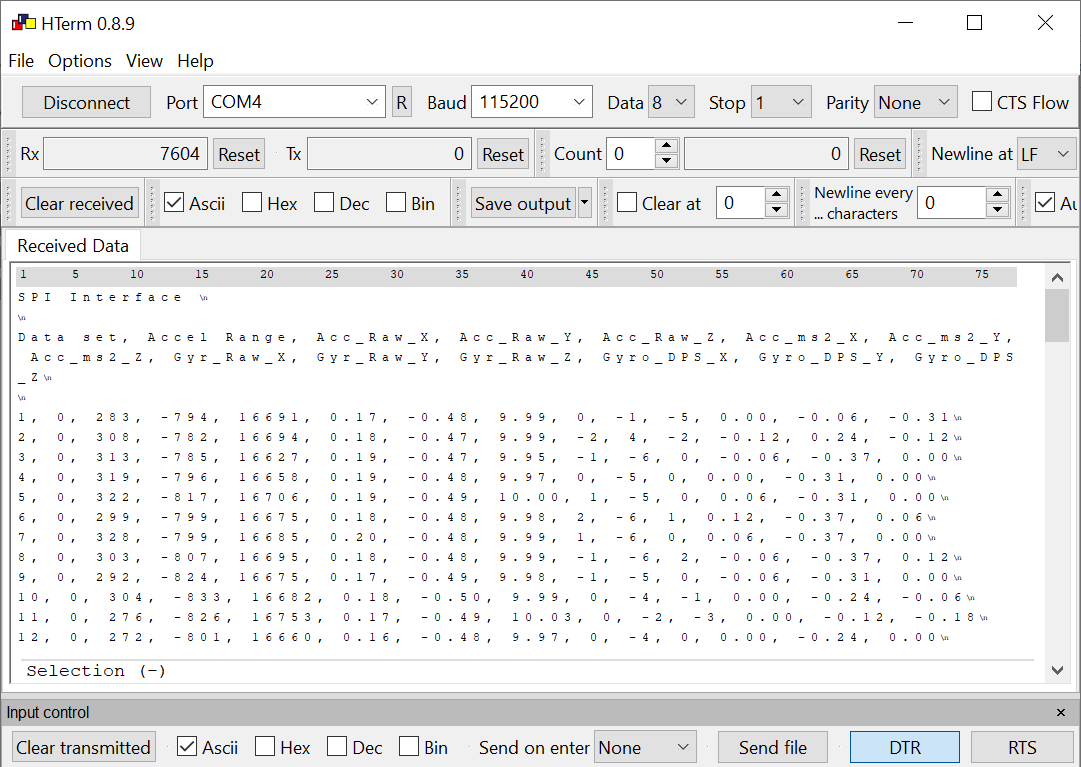
\includegraphics[width=0.9\textwidth]{coinesAPI_images/Mcu_example_output.png}
		\end{center}
	\end{figure}
	\begin{figure}[H]
		\begin{center}
			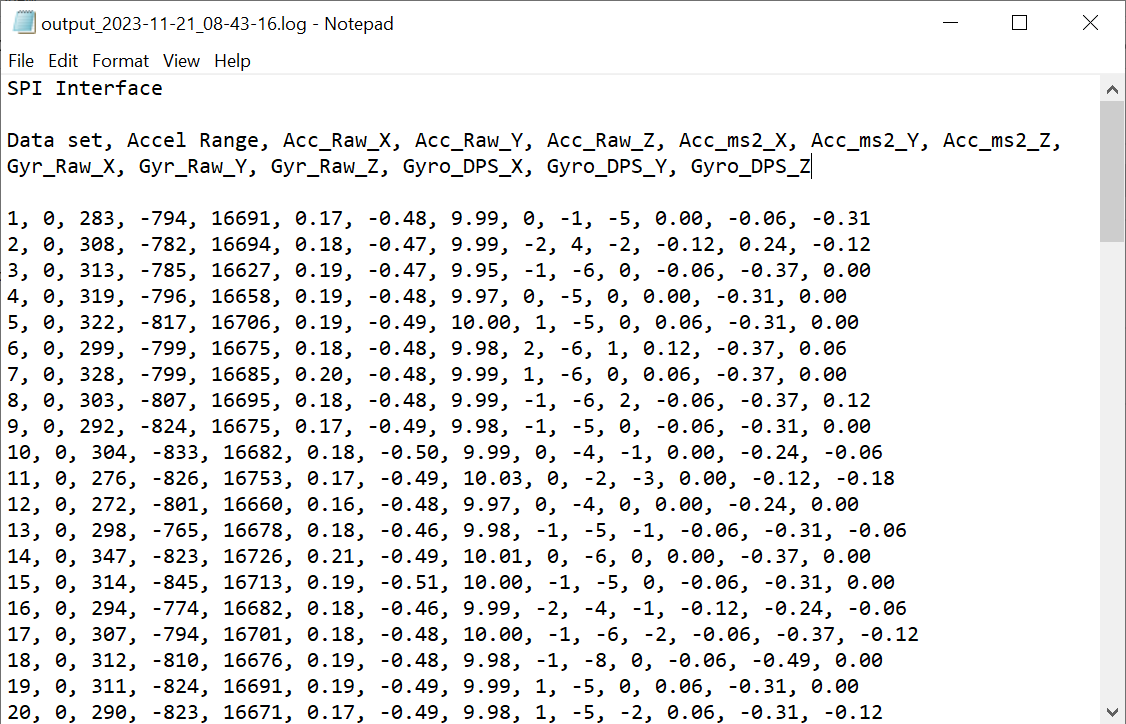
\includegraphics[width=0.9\textwidth]{coinesAPI_images/Mcu_example_log.png}
		\end{center}
	\end{figure}
\end{enumerate}
\subsection{Running example on MCU side via BLE}
The sequence of actions required for interfacing via BLE includes the steps below:
\begin{enumerate}
	\item Go to the \path{examples} folder in file explorer
	\item Open the common.c file in the selected example folder in your IDE
	\item Change COINES\_COMM\_INTF\_USB  to COINES\_COMM\_INTF\_BLE
	\begin{figure}[H]
		\begin{center}
			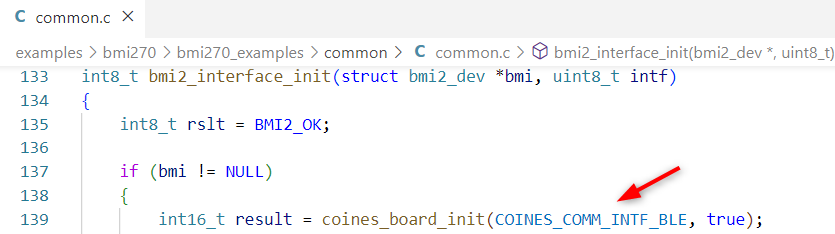
\includegraphics[width=0.9\textwidth]{coinesAPI_images/Mcu_example_ble_intf.png}
		\end{center}
	\end{figure}
	\item Open example script and change the 
	\begin{verbatim}
	printf(...) to fprintf(bt_w,...)
	\end{verbatim}
	\begin{figure}[H]
		\begin{center}
			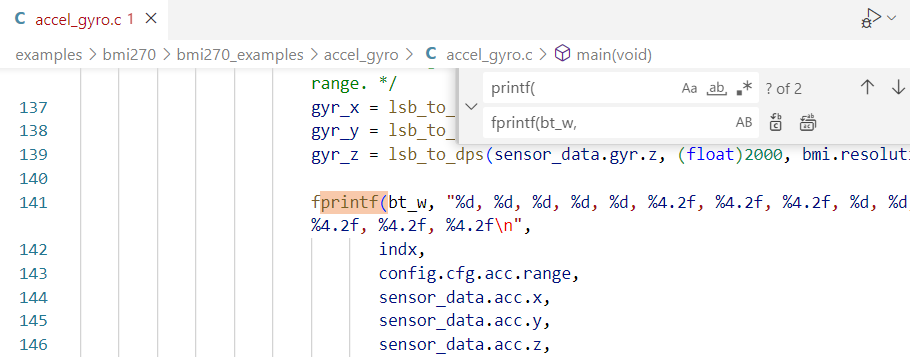
\includegraphics[width=0.9\textwidth]{coinesAPI_images/Mcu_example_ble_print.png}
		\end{center}
	\end{figure}
	\item Now follow the same steps from 1 - 4 in the above section.
	\item Connect the Application board to another power source and keep it within the BLE range.
	\item View the output in the \href{https://wiki.makerdiary.com/web-device-cli/}{Web Device CLI} site in your browser by connecting to board via BLE.
	\begin{figure}[H]
		\begin{center}
			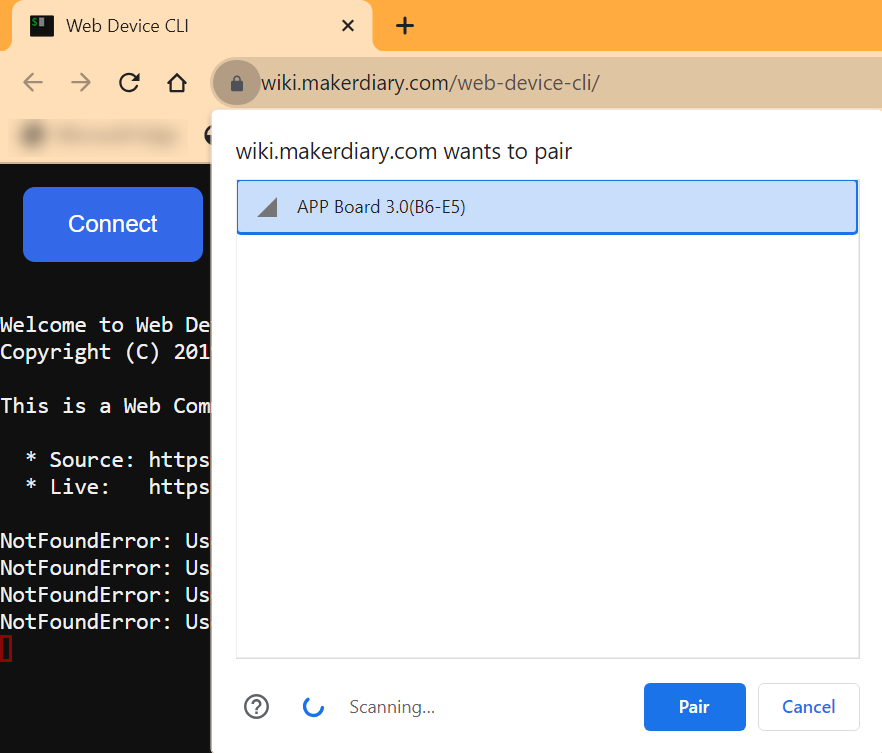
\includegraphics[width=0.7\textwidth]{coinesAPI_images/Mcu_example_ble_pair.png}
		\end{center}
	\end{figure}
	\begin{figure}[H]
		\begin{center}
			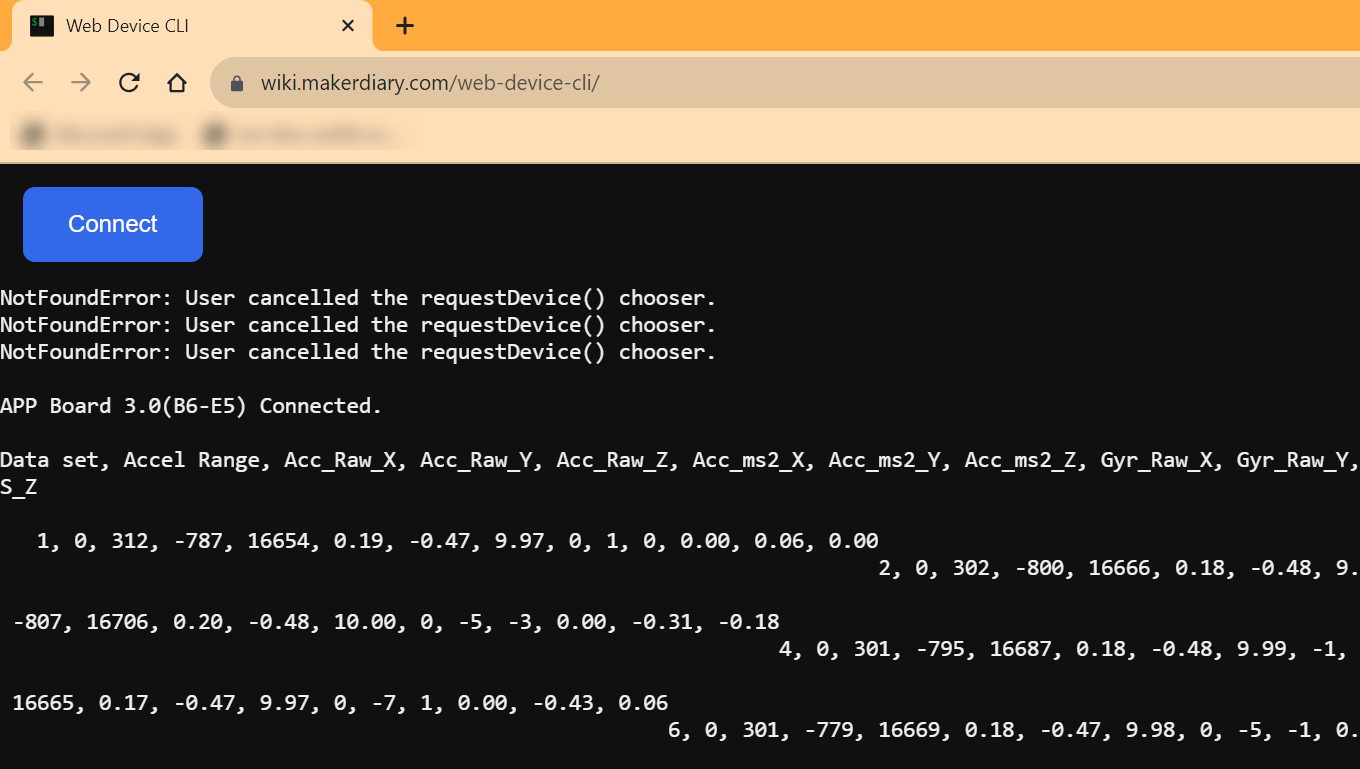
\includegraphics[width=0.9\textwidth]{coinesAPI_images/Mcu_example_ble_output.png}
		\end{center}
	\end{figure}
\end{enumerate}


\subsection{Running example on PC side}
Here are the step-by-step instructions to run examples on PC side:
\begin{itemize}
	\item Selected Platform: Windows
	\item Board: APP3.1
	\item Sensor shuttle: BMI270
	\item Example: \path{\examples\bmi270\bmi270_examples\step_counter}
\end{itemize}
\begin{enumerate}
	\item Connect the Application Board board via USB, with the sensor shuttle board mounted.
	\item Refer to section \ref{firmwareUpdate} and update the Coines Bridge firmware to the board.
	\item Open the command prompt or the terminal.
	\item Use the command \texttt{cd} to go to the directory where the example that is to be built is located.
	\begin{figure}[H]
		\begin{center}
			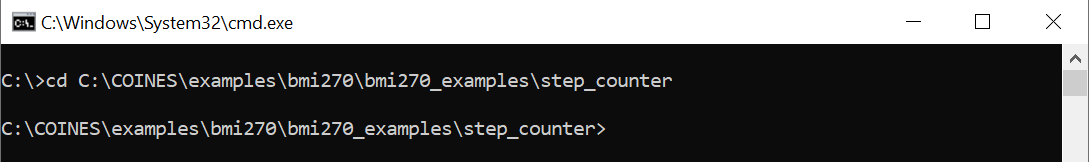
\includegraphics[width=0.9\textwidth]{coinesAPI_images/Pc_example_cd.png}
		\end{center}
	\end{figure}
	\item Execute command "mingw32-make TARGET=PC COINES\_BACKEND=COINES\_BRIDGE"
	\begin{figure}[H]
		\begin{center}
			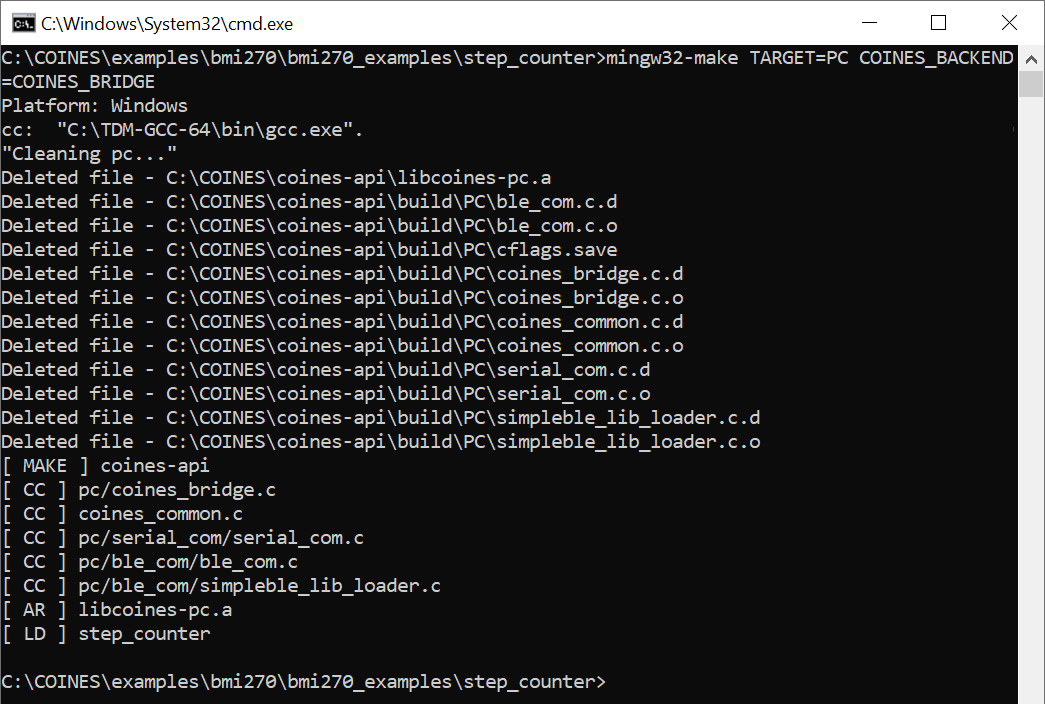
\includegraphics[width=0.9\textwidth]{coinesAPI_images/Pc_example_compile.png}
		\end{center}
	\end{figure}
	\item View the output in the command prompt by running the example executable.
	\begin{figure}[H]
		\begin{center}
			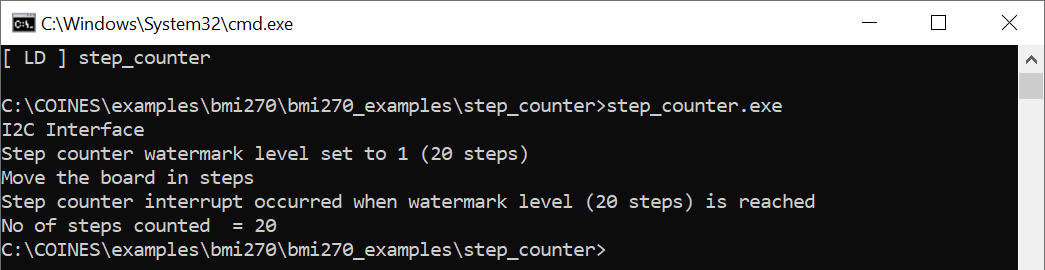
\includegraphics[width=0.9\textwidth]{coinesAPI_images/Pc_example_output.png}
		\end{center}
	\end{figure}
\end{enumerate}

\subsection{Running example on PC side via BLE}
The sequence of actions required for interfacing via BLE includes the steps below:
\begin{enumerate}
	\item Go to the examples folder in file explorer.
	\item Open the common.c file in the selected example folder in your IDE.
	\item Change COINES\_COMM\_INTF\_USB  to COINES\_COMM\_INTF\_BLE.
	\item Connect the Application board to another power source and keep it within the BLE range.
	\item Now follow the same steps from 3 - 6 in the above section.
	\begin{figure}[H]
		\begin{center}
			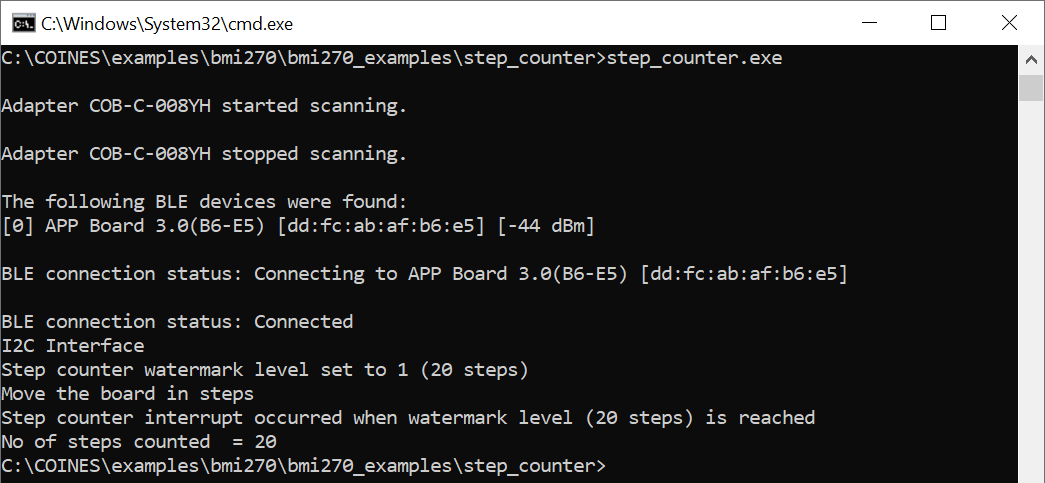
\includegraphics[width=0.9\textwidth]{coinesAPI_images/Pc_example_ble_output.png}
		\end{center}
	\end{figure}
\end{enumerate}
\newpage
\section{Examples on how to use COINES}
\subsection{COINES C examples}
\subsubsection{Establishing communication}
The following code snippet shows how to set up a connection with the board.
\begin{lstlisting}[language=c]
	#include <stdio.h>
	#include <stdlib.h>
	
	#include "coines.h"
	
	int main(void)
	{
		int8_t error_code;
		enum coines_comm_intf comm_intf = COINES_COMM_INTF_USB;

		error_code = coines_open_comm_intf(comm_intf, NULL);
		if (error_code == COINES_SUCCESS)
		{
			printf("\nSuccessfully connected to board!\n");
		}
		else
		{
			printf("\nUnable to connect with board!\n");
			exit(error_code);
		}
	
		coines_close_comm_intf(comm_intf, NULL);
	
		return 0;
	}

\end{lstlisting}
The APIs below can be used for board interface.
\begin{itemize}
	\item \texttt{coines\_open\_comm\_intf}
	\item \texttt{coines\_close\_comm\_intf}
\end{itemize}

\subsubsection{Getting board info}
The following code snippet shows how to get board information.
\begin{lstlisting}[language=c]
	#include <stdio.h>
	#include <stdlib.h>
	
	#include "coines.h"
	
	int main(void)
	{
		int8_t error_code;
		struct coines_board_info board_info;
		enum coines_comm_intf comm_intf = COINES_COMM_INTF_USB;
	
		error_code = coines_open_comm_intf(comm_intf, NULL);
		if (error_code < COINES_SUCCESS)
		{
			printf("\nUnable to connect with board!\n");
			exit(error_code);
		}
	
		error_code = coines_get_board_info(&board_info);
		if (error_code == COINES_SUCCESS)
		{
			printf("\nBoard Info:");
			printf("\n\tboard_info.board:0x%02X", board_info.board);
			printf("\n\tboard_info.hardware_id:0x%02X", board_info.hardware_id);
			printf("\n\tboard_info.shuttle_id:0x%02X", board_info.shuttle_id);
			printf("\n\tboard_info.software_id:0x%02X", board_info.software_id);
		}
	
		coines_close_comm_intf(comm_intf, NULL);
	
		return 0;
	}
	
\end{lstlisting}

\subsubsection{I2C config and read}
This basic program shows how to configure and perform I2C read.
\newline Sensor: BMI270
\begin{lstlisting}[language=c]
	#include <stdio.h>
	#include <stdlib.h>
	
	#include "coines.h"
	
	#define BMI2_I2C_PRIM_ADDR  0x68
	
	int main(void)
	{
		int8_t error_code;
		uint8_t chip_id;
		uint8_t reg_addr = 0x0;
		enum coines_comm_intf comm_intf = COINES_COMM_INTF_USB;
	
		error_code = coines_open_comm_intf(comm_intf, NULL);
		if (error_code == COINES_SUCCESS)
		{
			printf("\nSuccessfully connected to board!\n");
		}
		else
		{
			printf("\nUnable to connect with board!\n");
			exit(error_code);
		}
	
		/* Power up the board */
		(void)coines_set_shuttleboard_vdd_vddio_config(3300, 3300);
		coines_delay_usec(200);
	
		/* SDO to Ground */
		coines_set_pin_config(COINES_SHUTTLE_PIN_22, COINES_PIN_DIRECTION_OUT, COINES_PIN_VALUE_LOW);
	
		/* Make CSB pin HIGH */
		coines_set_pin_config(COINES_SHUTTLE_PIN_21, COINES_PIN_DIRECTION_OUT, COINES_PIN_VALUE_HIGH);
		coines_delay_msec(100);
	
		/* SDO pin is made low */
		coines_set_pin_config(COINES_SHUTTLE_PIN_SDO, COINES_PIN_DIRECTION_OUT, COINES_PIN_VALUE_LOW);
	
		/* I2C config */
		coines_config_i2c_bus(COINES_I2C_BUS_0, COINES_I2C_STANDARD_MODE);
	
		/* I2C read */
		(void)coines_read_i2c(COINES_I2C_BUS_0, BMI2_I2C_PRIM_ADDR, reg_addr, &chip_id, 1);
	
		printf("I2C read: Sensor chip ID - 0x%x\n", chip_id);
	
		(void)coines_set_shuttleboard_vdd_vddio_config(0, 0);
		coines_delay_msec(100);
	
		/* Coines interface reset */
		coines_soft_reset();
		coines_delay_msec(100);
	
		coines_close_comm_intf(comm_intf, NULL);
	
		return 0;
	}
\end{lstlisting}
The user shall pass GPIO pin numbers, read register address and I2C device address for sensors based on the selected sensor shuttle board. I2C communication require the proper setting of VDD and VDDIO using \texttt{coines\_set\_shuttleboard\_vdd\_vddio\_config}.
The APIs below can be used for I2C configure/read/write.
\begin{itemize}
	\item \texttt{coines\_config\_i2c\_bus}
	\item \texttt{coines\_read\_i2c}
	\item \texttt{coines\_write\_i2c}
\end{itemize}

\subsubsection{SPI config and read}
This basic program shows how to configure and perform SPI read.
\newline Sensor: BMI270
\begin{lstlisting}[language=c]
	#include <stdio.h>
	#include <stdlib.h>
	
	#include "coines.h"
	
	#define BMI2_SPI_RD_MASK  0x80
	
	int main(void)
	{
		int8_t error_code;
		uint8_t chip_id[2], dummy_byte;
	
		/* An extra dummy byte is read during SPI read */
		uint8_t dummy_byte_len = 1;
		uint8_t reg_addr = 0x0;
		enum coines_comm_intf comm_intf = COINES_COMM_INTF_USB;
	
		error_code = coines_open_comm_intf(comm_intf, NULL);
		if (error_code == COINES_SUCCESS)
		{
			printf("\nSuccessfully connected to board!\n");
		}
		else
		{
			printf("\nUnable to connect with board!\n");
			exit(error_code);
		}
	
		/* Power up the board */
		coines_set_shuttleboard_vdd_vddio_config(3300, 3300);
		coines_delay_msec(200);
	
		/* SPI config */
		(void)coines_config_spi_bus(COINES_SPI_BUS_0, COINES_SPI_SPEED_5_MHZ, COINES_SPI_MODE3);
	
		/* Pin config */
		coines_set_pin_config(COINES_SHUTTLE_PIN_21, COINES_PIN_DIRECTION_OUT, COINES_PIN_VALUE_HIGH);
	
		/* Mask read register address for SPI */
		reg_addr = (reg_addr | BMI2_SPI_RD_MASK);
	
		/* Dummy read for SPI init*/
		(void)coines_read_spi(COINES_SPI_BUS_0, COINES_MINI_SHUTTLE_PIN_2_1, reg_addr, &dummy_byte, 1);
		coines_delay_usec(450);
	
		/* SPI read */
		(void)coines_read_spi(COINES_SPI_BUS_0, COINES_MINI_SHUTTLE_PIN_2_1, reg_addr, chip_id, 1 + dummy_byte_len);
		coines_delay_usec(450);
	
		printf("SPI read: Sensor chip ID - 0x%x\n", chip_id[dummy_byte_len]);
	
		(void)coines_set_shuttleboard_vdd_vddio_config(0, 0);
		coines_delay_msec(100);
	
		/* Coines interface reset */
		coines_soft_reset();
		coines_delay_msec(100);
	
		coines_close_comm_intf(comm_intf, NULL);
	
		return 0;
	}
\end{lstlisting}
The user shall pass GPIO pin numbers, read register address and SPI CS pins for sensors based on the selected sensor shuttle board. SPI communication require the proper setting of VDD and VDDIO using \texttt{coines\_set\_shuttleboard\_vdd\_vddio\_config}.
The APIs below can be used for SPI configure/read/write.
\begin{itemize}
	\item \texttt{coines\_config\_spi\_bus}
	\item \texttt{coines\_read\_spi}
	\item \texttt{coines\_write\_spi}
\end{itemize}
\subsubsection{Led and button control}
The example program below is to control LEDs and buttons on the board.
\newline Target: MCU
\begin{lstlisting}[language=c]
	#include <stdio.h>
	#include <stdbool.h>
	#include "coines.h"
	
	/* Callback for button 1 interrupt */
	static void button1CB(uint32_t param1, uint32_t param2);
	
	/*Callback for button 1 event */
	void button1CB(uint32_t param1, uint32_t param2)
	{
		(void)param1;
		(void)param2;
	
		coines_set_led(COINES_LED_RED, COINES_LED_STATE_ON);
		coines_set_led(COINES_LED_GREEN, COINES_LED_STATE_OFF);
		coines_set_led(COINES_LED_BLUE, COINES_LED_STATE_ON);
	}
	
	int main(void)
	{
		coines_open_comm_intf(COINES_COMM_INTF_USB, NULL);
	
		coines_set_pin_config(COINES_APP30_BUTTON_1, COINES_PIN_DIRECTION_IN, COINES_PIN_VALUE_HIGH);
		coines_attach_interrupt(COINES_APP30_BUTTON_1, button1CB, COINES_PIN_INTERRUPT_FALLING_EDGE);
	
		coines_close_comm_intf(COINES_COMM_INTF_USB, NULL);
	
		return 0;
	}
\end{lstlisting}

\subsubsection{File listing in External memory}
To list the files in the external memory, below snippet can be used.
\newline Target: MCU
\begin{lstlisting}[language=c]
	#include <stdio.h>
	#include "coines.h"
	
	int main(void)
	{
		coines_open_comm_intf(COINES_COMM_INTF_USB, NULL);
		DIR *directory;
		struct dirent *dir;
		directory = opendir(".");
		if (directory)
		{
			while ((dir = readdir(directory)) != NULL)
			{
				printf("%s\n", dir->d_name);
			}
	
			closedir(directory);
		}
	
		coines_close_comm_intf(COINES_COMM_INTF_USB, NULL);
	
		return 0;
	}
\end{lstlisting}
\subsubsection{Temperature measurement}
This simple program demonstrates how to measure temperature of the board.
\newline Target: MCU
\begin{lstlisting}[language=c]
	#include <stdio.h>
	#include <stdlib.h>

	#include "coines.h"

	int main(void)
	{
		int8_t error_code;
		float temp_data = 0;
		enum coines_comm_intf comm_intf = COINES_COMM_INTF_USB;

		error_code = coines_open_comm_intf(comm_intf, NULL);
		if (error_code == COINES_SUCCESS)
		{
			printf("\nSuccessfully connected to board!\n");
		}
		else
		{
			printf("\nUnable to connect with board!\n");
			exit(error_code);
		}

		/* Power up the board */
		coines_set_shuttleboard_vdd_vddio_config(1800, 1800);
		coines_delay_msec(200);

		/* Read temperature data */
		coines_read_temp_data(&temp_data);
		printf("\nTemperature data = %f in degC", temp_data);

		coines_set_shuttleboard_vdd_vddio_config(0, 0);
		coines_delay_msec(100);

		coines_close_comm_intf(comm_intf, NULL);

		return 0;
	}
\end{lstlisting}

\subsubsection{Battery level measurement}
This simple program demonstrates how to measure battery level when a battery is connected to the board.
\newline Target: MCU
\begin{lstlisting}[language=c]
	#include <stdio.h>
	#include <stdlib.h>
	
	#include "coines.h"
	
	int main(void)
	{
		int8_t error_code;
		uint8_t batt_status_percentage = 0;
		uint16_t batt_status_in_milli_volts = 0;
		enum coines_comm_intf comm_intf = COINES_COMM_INTF_BLE;
	
		error_code = coines_open_comm_intf(comm_intf, NULL);
		if (error_code == COINES_SUCCESS)
		{
			printf("\nSuccessfully connected to board!\n");
		}
		else
		{
			printf("\nUnable to connect with board!\n");
			exit(error_code);
		}
	
		/* Read battery level */
		coines_read_bat_status(&batt_status_in_milli_volts, &batt_status_percentage);
		fprintf(bt_w, "Battery level in percentage = %d %% \r\n", batt_status_percentage);
		fprintf(bt_w, "Battery level in millivolts = %d mV \r\n", batt_status_in_milli_volts);
	
		coines_close_comm_intf(comm_intf, NULL);
	
		return 0;
	}
\end{lstlisting}

\subsubsection{Configure BLE communication}\label{bleComConfig}
This example shows how to configure BLE connection.
\newline Target: PC
\begin{lstlisting}[language=c]
	#include <stdio.h>
	#include <string.h>
	#include <stdlib.h>
	
	#include "coines.h"
	
	/*! Macros to hold the BLE peripheral name and address to be connected */
	/*! Please change the name and address with BLE name of the Application board under test */
	#define BLE_NAME  "APP Board 3.0(B6-E5)"
	#define BLE_ADDR  "dd:fc:ab:af:b6:e5"
	
	/*! Variable to hold the communication interface type */
	const enum coines_comm_intf comm_intf = COINES_COMM_INTF_BLE;
	
	int main(void)
	{
		struct ble_peripheral_info ble_config = { BLE_ADDR, "" };
		struct ble_peripheral_info ble_info[40];
		uint8_t peripheral_count, i;
		int8_t result;
	
		/* Get the BLE peripheral list */
		result = coines_scan_ble_devices(ble_info, &peripheral_count, 7000);
		if (result != COINES_SUCCESS)
		{
			const char *err_str = get_coines_error_str(result);
			printf("\n%s", err_str);
			exit(result);
		}
	
		/* Print the BLE peripheral list */
		printf("\nBLE devices found:");
		for (i = 0; i < peripheral_count; i++)
		{
			printf("\n[%d] %s [%s]", i, ble_info[i].ble_identifier, ble_info[i].ble_address);
		}
	
		/* Open BLE connection */
		result = coines_open_comm_intf(comm_intf, &ble_config);
		if (result == COINES_SUCCESS)
		{
			printf("\nSuccessfully connected to board!\n");
		}
		else
		{
			printf("\nUnable to connect with board!\n");
			exit(result);
		}
	
		/* Close BLE connection */
		coines_soft_reset();
		coines_delay_msec(100);
	
		coines_close_comm_intf(comm_intf, NULL);
	
		return 0;
	}	

\end{lstlisting}
The user shall modify BLE settings like address and name before executing this example.
\subsubsection{Configure Serial communication}\label{serialComConfig}
This example shows how to configure Serial COM connection.
\newline Target: PC
\begin{lstlisting}[language=c]
	#include <stdio.h>
	#include <string.h>
	#include <stdlib.h>
	
	#include "coines.h"
	
	#define ROBERT_BOSCH_USB_VID   (0x108C)
	#define ARDUINO_USB_VID        (0x2341)
	#define BST_APP30_CDC_USB_PID  (0xAB3C)
	#define BST_APP20_CDC_USB_PID  (0xAB2C)
	#define ARDUINO_NICLA_USB_PID  (0x0060)
	
	/*! Variable to hold the communication interface type */
	const enum coines_comm_intf comm_intf = COINES_COMM_INTF_USB;
	
	int main(void)
	{
		int16_t result;
		struct coines_serial_com_config scom_config;
	
		scom_config.baud_rate = 38400;
		scom_config.vendor_id = ROBERT_BOSCH_USB_VID;
		scom_config.product_id = BST_APP30_CDC_USB_PID;
		scom_config.com_port_name = "COM4";
		scom_config.rx_buffer_size = 2048;
	
		/* Open serial connection */
		result = coines_open_comm_intf(comm_intf, &scom_config);
		if (result == COINES_SUCCESS)
		{
			printf("\nSuccessfully connected to board!\n");
		}
		else
		{
			printf("\nUnable to connect with board!\n");
			exit(result);
		}
	
		/* Close serial connection */
		coines_soft_reset();
		coines_delay_msec(100);
	
		coines_close_comm_intf(comm_intf, NULL);
	
		return 0;
	}
	
\end{lstlisting}
The user shall modify Serial COM settings like vendor ID, product ID and COM port name before executing this example.
\subsection{COINES Python examples}

\subsubsection{Getting board info}\label{GettingBoardInfo}
The following code snippet shows how to get board information.
\begin{lstlisting}[language=python]
	import coinespy as cpy
	from coinespy import ErrorCodes
	
	COM_INTF = cpy.CommInterface.USB
	
	if __name__ == "__main__":
		board = cpy.CoinesBoard()
		print('coinespy version - %s' % cpy.__version__)
		board.open_comm_interface(COM_INTF)
		if board.error_code != ErrorCodes.COINES_SUCCESS:
			print(f'Could not connect to board: {board.error_code}')
		else:
			b_info = board.get_board_info()
			print(f"coines lib version: {board.lib_version}")
			print(
				f'BoardInfo: HW/SW ID: {hex(b_info.HardwareId)}/{hex(b_info.SoftwareId)}')
			board.close_comm_interface()
\end{lstlisting}

\subsubsection{I2C config and read}
This basic program shows how to configure and perform I2C read.
\newline Sensor: BMI085
\begin{lstlisting}[language=python]
	import sys
	import time
	import coinespy as cpy
	from coinespy import ErrorCodes

	COM_INTF = cpy.CommInterface.USB
	
	if __name__ == "__main__":
		BOARD = cpy.CoinesBoard()

		BOARD.open_comm_interface(COM_INTF)
		if BOARD.error_code != ErrorCodes.COINES_SUCCESS:
			print(f"Open Communication interface: {BOARD.error_code}")
			sys.exit()
	
		BMI085_I2C_ADDRESS_ACCEL = 0x18
		BMI085_I2C_ADDRESS_GYRO  = 0x68
		BMI08_REG_ACCEL_CHIP_ID = 0x00
	
		BOARD.set_shuttleboard_vdd_vddio_config(vdd_val=0, vddio_val=0)
	
		#  Config I2C pins
		BOARD.set_pin_config(
			cpy.MultiIOPin.SHUTTLE_PIN_8, cpy.PinDirection.OUTPUT, cpy.PinValue.LOW)
		BOARD.set_pin_config(
			cpy.MultiIOPin.SHUTTLE_PIN_SDO, cpy.PinDirection.OUTPUT, cpy.PinValue.LOW)
		# Set PS pin of gyro to HIGH for proper protocol selection
		BOARD.set_pin_config(
			cpy.MultiIOPin.SHUTTLE_PIN_9, cpy.PinDirection.OUTPUT, cpy.PinValue.HIGH)
	
		# I2C config
		BOARD.config_i2c_bus(
			cpy.I2CBus.BUS_I2C_0, BMI085_I2C_ADDRESS_ACCEL, cpy.I2CMode.STANDARD_MODE)
	
		BOARD.set_shuttleboard_vdd_vddio_config(vdd_val=3.3, vddio_val=3.3)
		time.sleep(0.2)
	
		# I2C read
		accel_chip_id = BOARD.read_i2c(
			cpy.I2CBus.BUS_I2C_0, BMI08_REG_ACCEL_CHIP_ID, 1, BMI085_I2C_ADDRESS_ACCEL)
		gyro_chip_id = BOARD.read_i2c(
			cpy.I2CBus.BUS_I2C_0, BMI08_REG_ACCEL_CHIP_ID, 1, BMI085_I2C_ADDRESS_GYRO)
	
		print(f"Accel chip id: {hex(accel_chip_id[0])}")
		print(f"Gyro chip id: {hex(gyro_chip_id[0])}")
	
		# Deinit board
		BOARD.set_shuttleboard_vdd_vddio_config(vdd_val=0, vddio_val=0)
		BOARD.soft_reset()
	
		BOARD.close_comm_interface()	
\end{lstlisting}
The user shall pass GPIO pin numbers, read register address and I2C device address for sensors based on the selected sensor shuttle board. I2C communication require the proper setting of VDD and VDDIO using \texttt{set\_shuttleboard\_vdd\_vddio\_config}.

\subsubsection{SPI config and read}
This basic program shows how to configure and perform SPI read.
\newline Sensor: BMI085
\begin{lstlisting}[language=python]
	import sys
	import time
	import coinespy as cpy
	from coinespy import ErrorCodes
	
	COM_INTF = cpy.CommInterface.USB
	
	if __name__ == "__main__":
		BOARD = cpy.CoinesBoard()

		BOARD.open_comm_interface(COM_INTF)
		if BOARD.error_code != ErrorCodes.COINES_SUCCESS:
			print(f"Open Communication interface: {BOARD.error_code}")
			sys.exit()
	
		BMI085_ACCEL_CS_PIN = cpy.MultiIOPin.SHUTTLE_PIN_8
		BMI085_GYRO_CS_PIN = cpy.MultiIOPin.SHUTTLE_PIN_14
		BMI08_REG_ACCEL_CHIP_ID = 0x00
		accel_dummy_byte_len = 1
	
		BOARD.set_shuttleboard_vdd_vddio_config(vdd_val=0, vddio_val=0)
	
		# Config CS pin
		BOARD.set_pin_config(
			BMI085_ACCEL_CS_PIN, cpy.PinDirection.OUTPUT, cpy.PinValue.HIGH)
		BOARD.set_pin_config(
			BMI085_GYRO_CS_PIN, cpy.PinDirection.OUTPUT, cpy.PinValue.HIGH)
		# Set PS pin of gyro to LOW for proper protocol selection
		BOARD.set_pin_config(
			cpy.MultiIOPin.SHUTTLE_PIN_9, cpy.PinDirection.OUTPUT, cpy.PinValue.LOW)
	
		#  SPI config
		BOARD.config_spi_bus(cpy.SPIBus.BUS_SPI_0, BMI085_ACCEL_CS_PIN,
							 cpy.SPISpeed.SPI_1_MHZ, cpy.SPIMode.MODE0)
	
		BOARD.set_shuttleboard_vdd_vddio_config(vdd_val=3.3, vddio_val=3.3)
		time.sleep(0.2)
	
		# Initialize SPI by dummy read
		reg_data = BOARD.read_spi(cpy.SPIBus.BUS_SPI_0, BMI08_REG_ACCEL_CHIP_ID, 1)
	
		# SPI read
		accel_chip_id = BOARD.read_spi(
			cpy.SPIBus.BUS_SPI_0, BMI08_REG_ACCEL_CHIP_ID, 1 + accel_dummy_byte_len, BMI085_ACCEL_CS_PIN)
		gyro_chip_id = BOARD.read_spi(
			cpy.SPIBus.BUS_SPI_0, BMI08_REG_ACCEL_CHIP_ID, 1, BMI085_GYRO_CS_PIN)
	
		print(f"Accel chip id: {hex(accel_chip_id[accel_dummy_byte_len])}")
		print(f"Gyro chip id: {hex(gyro_chip_id[0])}")
	
		# Deinit board
		BOARD.set_shuttleboard_vdd_vddio_config(vdd_val=0, vddio_val=0)
		BOARD.soft_reset()
	
		BOARD.close_comm_interface()
\end{lstlisting}
The user shall pass GPIO pin numbers, read register address and SPI CS pins for sensors based on the selected sensor shuttle board. SPI communication require the proper setting of VDD and VDDIO using \texttt{set\_shuttleboard\_vdd\_vddio\_config}.

\newpage
\section{Debugging via VS code}
Here are the steps to follow to debug programs via VS code:
\begin{itemize}
	\item Download Segger software from from \url{https://www.segger.com/downloads/jlink/}.
	\item Refer to \url{https://wiki.segger.com/J-Link_Visual_Studio_Code} for using J-link with VS code.
	\item Download the NRF5 .svd file from Nordic Semiconductor github.
	\item Connect J-link to SWD debugger connector.
	\begin{figure}[H]
		\begin{center}
			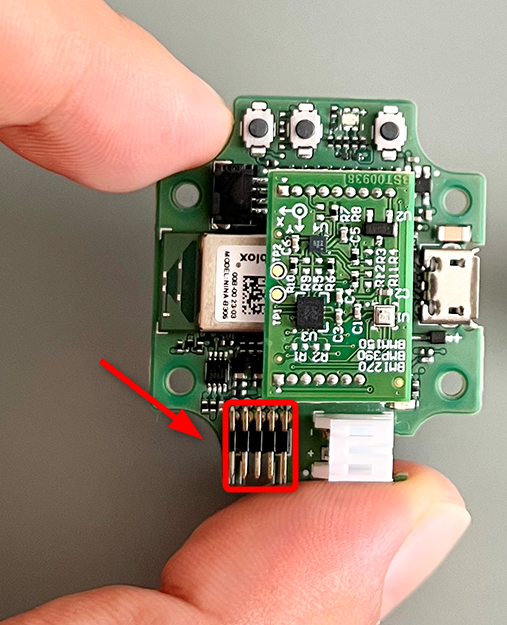
\includegraphics[width=0.25\textwidth]{coinesAPI_images/App31_jlink_connection.png}
			\caption{APP3.1 Debugger connector}
		\end{center}
	\end{figure}
	\item Below is the sample launch.json config for VS code debug.
	\begin{figure}[H]
		\begin{center}
			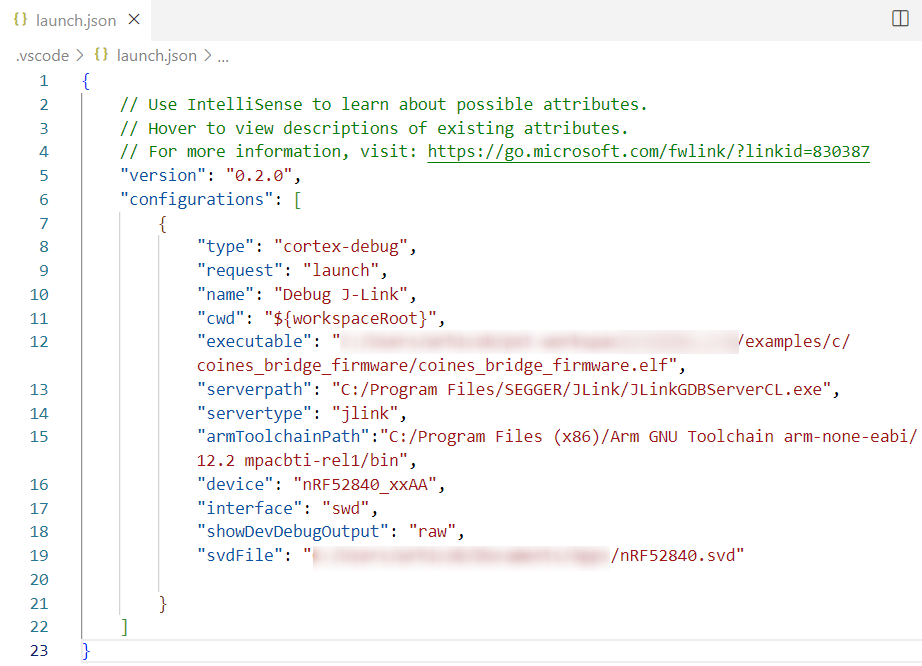
\includegraphics[width=0.8\textwidth]{coinesAPI_images/Debug_launch_json.png}
			\caption{VS code debug launch.json}
		\end{center}
	\end{figure}
\end{itemize}

\newpage
\section{Media Transfer Protocol (MTP) firmware for APP3.x}

The external memory chip W25M02/W25N02 on APP3.x is based on NAND flash.

FAT filesystem on NAND flash memory results in a complicated solution which uses of lot of RAM. Moreover use of FAT without Flash Translation Layer (to save RAM) wears out NAND flash with frequent usage. Hence the choice of \href{https://github.com/conservify/FLogFS}{FlogFS}, a filesystem optimized for use with NAND flash.

But the use of `FlogFS`, presents a new problem 'Filesystem access from PC via USB'. Use of `FlogFS` with USB Mass Storage protocol is not possible because operating system can't recognize `FlogFS` as a valid filesystem.

Use of custom protocol to do filesystem operations would mean re-inventing the wheel and a lot of effort. User also would not have the same experience as with USB Mass Storage.

Solution was to go with the "Media Transfer Protocol" developed initially by Microsoft for Portable Devices like MP3 players. Starting from Android Kitkat (v4.4), MTP is the only way to access files on an Android device since the whole flash memory (included user storage space) uses filesystems like ext4, YAFFS, F2FS, etc.,

Files in APP3.x's NAND flash memory can be viewed using the USB MTP firmware.

Supported on Windows, Linux, macOS and Android (via USB OTG).

\begin{figure}[H]
	\begin{center}
		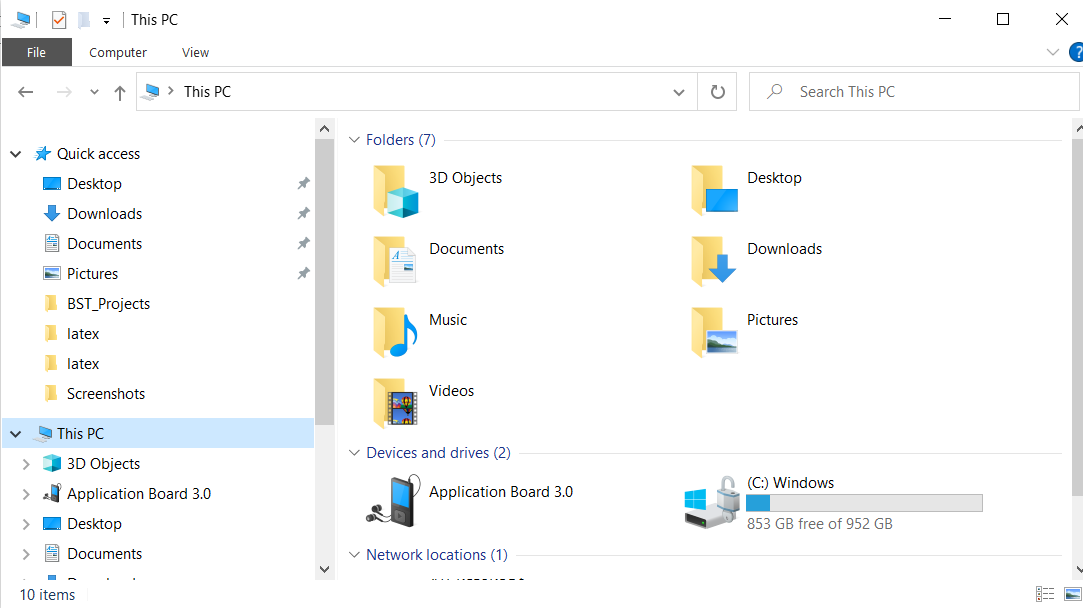
\includegraphics[width=0.7\textwidth]{coinesAPI_images/MTP_windows.png}
		\caption{APP3.x in MTP mode on Windows}
	\end{center}
\end{figure}

\begin{figure}[H]
	\begin{center}
		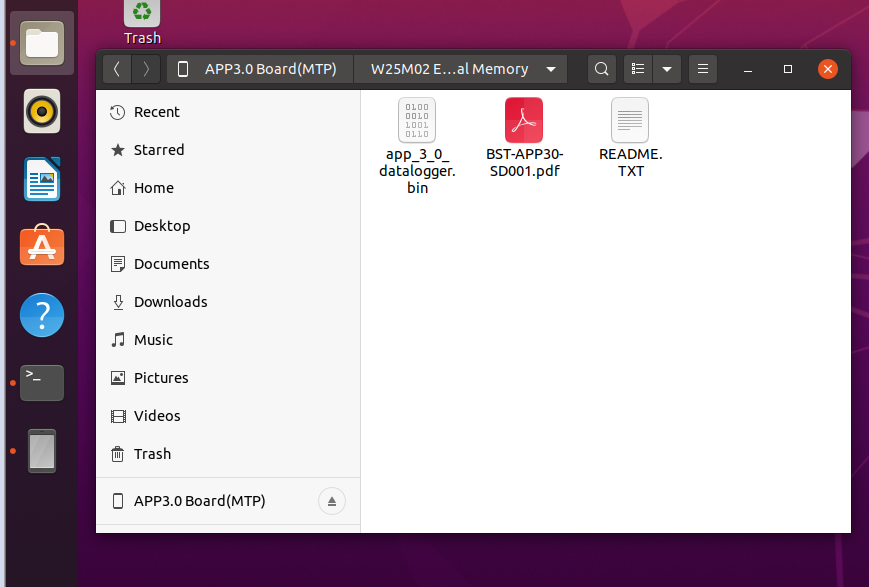
\includegraphics[width=0.7\textwidth]{coinesAPI_images/MTP_Ubuntu_Nautilus.png}
		\caption{APP3.x in MTP mode on Linux}
	\end{center}
\end{figure}

\begin{figure}[H]
	\begin{center}
		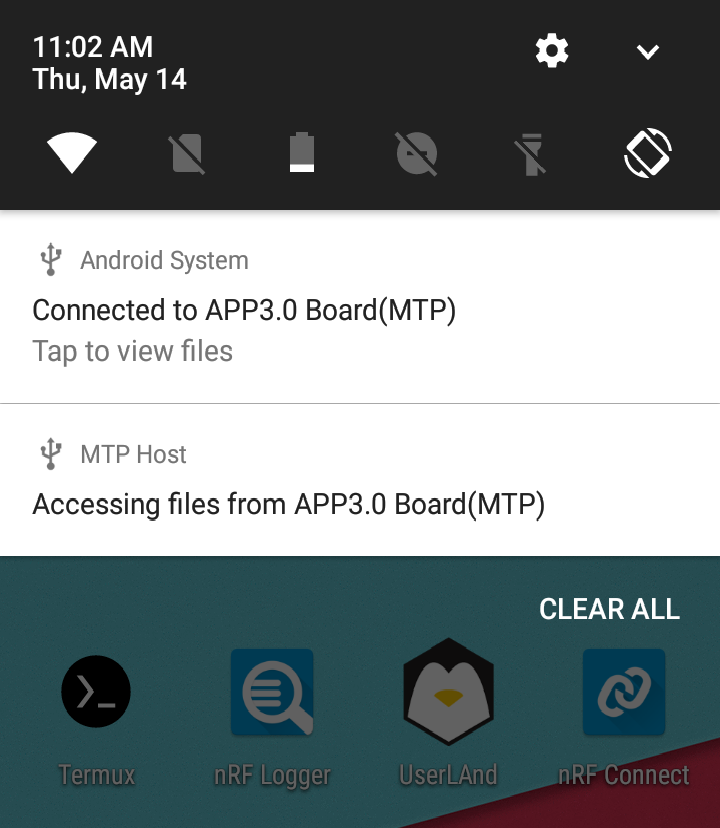
\includegraphics[width=0.5\textwidth]{coinesAPI_images/MTP_Android_2.png}
		\caption{APP3.x in MTP mode on Andriod}
	\end{center}
\end{figure}

\begin{figure}[H]
	\begin{center}
		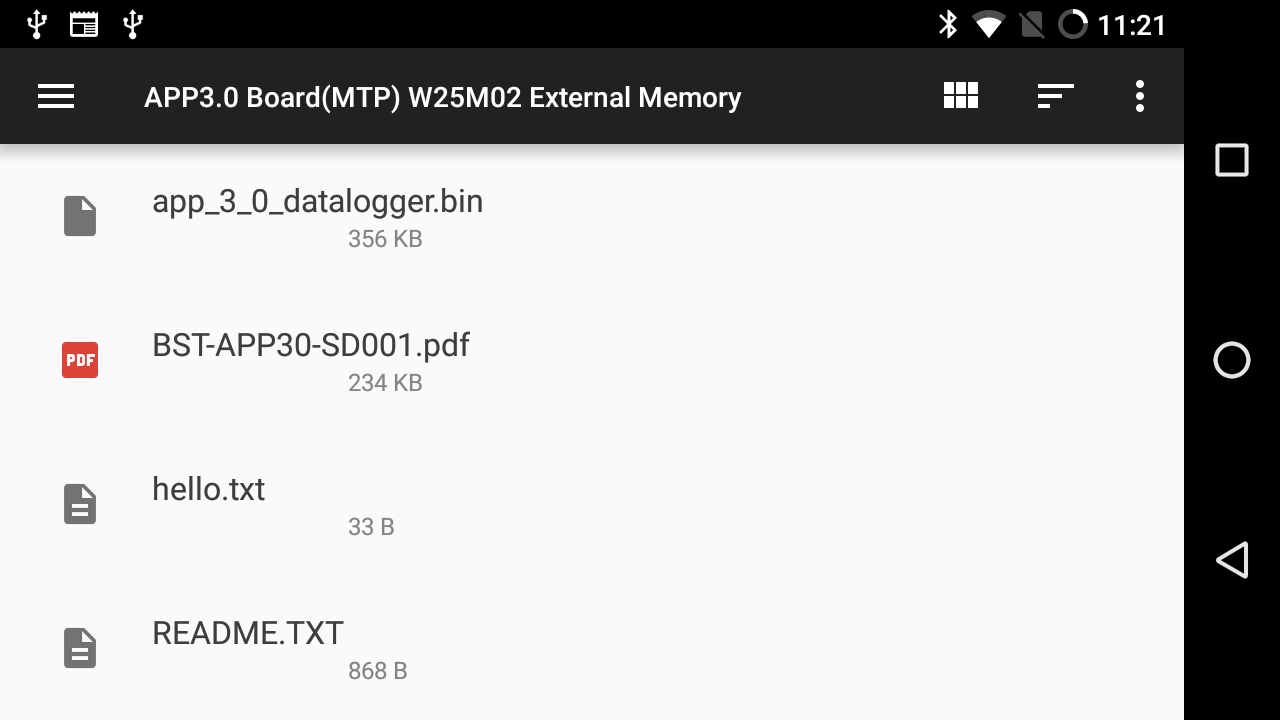
\includegraphics[width=0.7\textwidth]{coinesAPI_images/MTP_Android_3.png}
		\caption{Files in external memory listed on Andriod device}
	\end{center}
\end{figure}

\subsection{Copying the files using MTP}
The following procedure demonstrates how to copy files using MTP:
\begin{itemize}
	\item APP3.x comes with the preloaded MTP firmware update package.
	\item Refer to section \ref{SwitchModes} to switch to MTP mode
	\item The device will enumerate as an MTP device with name "Application Board 3.x". Click on it and select the "W25M02 External Memory"
	\item The device will list all the available files and all required files can be copied.
\end{itemize}

\begin{figure}[H]
	\begin{center}
		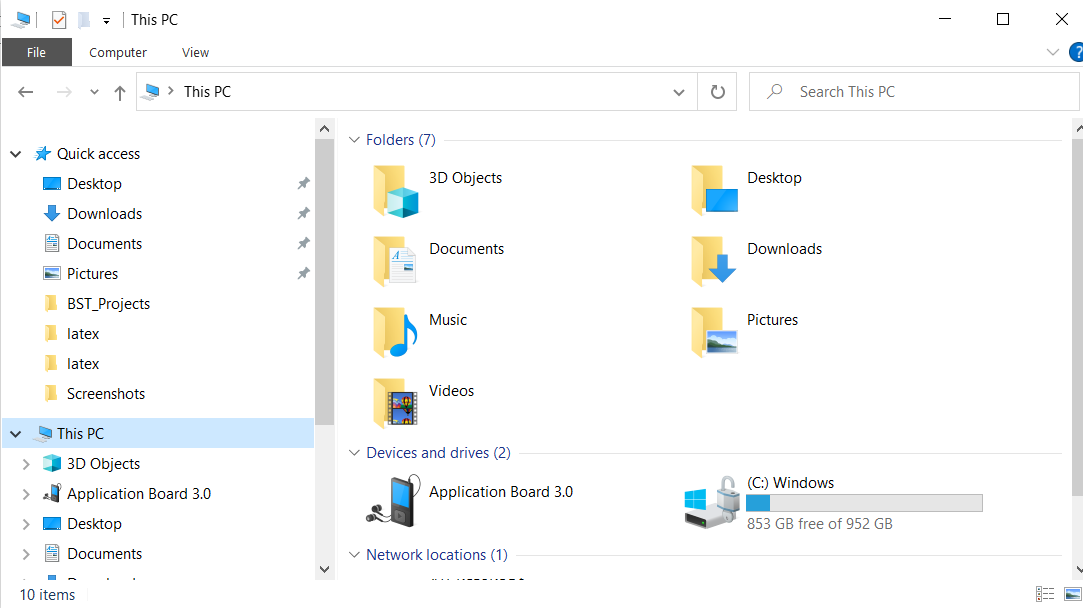
\includegraphics[width=0.7\textwidth]{coinesAPI_images/MTP_windows.png}
		\caption{Copy data log files to the PC over USB MTP}
	\end{center}
\end{figure}

\newpage
\section{USB/BLE DFU bootloader}

A USB/BLE  Bootloader for APP3.x/nRF52840 and Nicla Sense ME/nRF52832 chip comply with below items:

\begin{itemize}
	\item \url{https://www.usb.org/sites/default/files/DFU_1.1.pdf}
	\item \href{https://infocenter.nordicsemi.com/index.jsp?topic=%2Fcom.nordic.infocenter.sdk5.v15.2.0%2Fble_sdk_app_dfu_bootloader.html&cp=9_5_3_4_1_3}{nRF5 SDK v15.2.0 - BLE Secure DFU Bootloader}
\end{itemize}

\subsection{Key Features}

\subsubsection{USB DFU}
The key features of USB DFU are as follows:
\begin{itemize}
	\item Code download to RAM or FLASH
	\item Code read back (upload) from  RAM or FLASH (Useful for taking firmware backups)
	\item Works with Windows, Linux, macOS and Android.
\end{itemize}

\subsubsection{BLE DFU}
The key features of BLE DFU are as follows:
\begin{itemize}
	\item Code download to FLASH.
	\item Works with PC and mobile devices with iOS/Android.
\end{itemize}

Bootloader was written taking into account the following aspects:
\begin{itemize}
	\item Usability.
	\begin{enumerate}[label=\roman*.]
		\item No special driver installation or admin rights should be required.
		\item The update process should be straight forward.
	\end{enumerate}
	\item Maintainability
	\begin{enumerate}[label=\roman*.]
		\item Open source community takes care of PC side tools. For eg: dfu-util is a cross platform tool.
		\item Use Google Chrome's WebUSB to update firmware. Sample implementation \url{https://devanlai.github.io/webdfu/dfu-util/}
	\end{enumerate}
	\item Size
	\item COINES on MCU.
\end{itemize}

\subsection{Invoking the Bootloader}
\begin{enumerate}
	\item To invoke Bootloader from Hardware, switch the board to bootloader mode (refer to section \ref{SwitchModes}).
	\item To invoke Bootloader from Software, use the below snippets in your program based on the board selected.
\end{enumerate}

\begin{itemize}
	\item APP3.x
	\begin{enumerate}[label=\roman*.]
		\item Write 0x4E494F43 ('N','I','O','C') to MAGIC\_LOCATION (0x2003FFF4)
		\item Write 0x0 or 0xF0000 to APP\_START\_ADDR (0x2003FFF8)
		\item Call NVIC\_SystemReset()
		\begin{lstlisting}[language=C]
		
		#define  MAGIC_LOCATION (0x2003FFF4)
		#define  APP_START_ADDR (*(uint32_t *)(MAGIC_LOCATION+4)
		 
		*((uint32_t *)MAGIC_LOCATION) == 0x4E494F43;
		APP_START_ADDR = 0xF0000;
		//APP_START_ADDR = 0x0;
		NVIC_SystemReset();
		
		\end{lstlisting}
	\end{enumerate}
\end{itemize}

\begin{itemize}
	\item Nicla Sense ME Board
	\begin{enumerate}[label=\roman*.]
		\item Write 0x544F4F42 ('T','O','O','B') to MAGIC\_LOCATION (0x2000F804)
		\item Call NVIC\_SystemReset()
		\begin{lstlisting}[language=C]
		
		#define  MAGIC_LOCATION (0x2000F804)
		#define  APP_START_ADDR (*(uint32_t *)(MAGIC_LOCATION+4)
		 
		*((uint32_t *)MAGIC_LOCATION) == 0x544F4F42;
		NVIC_SystemReset();
		
		\end{lstlisting}
	\end{enumerate}
\end{itemize}
It is to be noted that the same feature can also be used to perform application switch ( 2 or more applications can reside in the same flash memory at different address locations ). Just write the application start address to APP\_START\_ADDR instead of bootloader address
\subsection{Using the Bootloader via USB}
The commands below demonstrate how to use dfu-util for different scenarios:

\begin{itemize}
	\item Path to dfu-util: \path{\tools\usb-dfu}
\end{itemize}

Write firmware to Flash memory using following command
\begin{itemize}
	\item dfu-util -a FLASH -D <firmware>.bin -R
\end{itemize}

Write firmware to RAM memory using following command
\begin{itemize}
	\item dfu-util -a RAM -D <firmware>.bin -R
\end{itemize}

Read firmware from Flash memory using following command
\begin{itemize}
	\item dfu-util -a FLASH -U <firmware>.bin
\end{itemize}

Read firmware from RAM memory using following command
\begin{itemize}
	\item dfu-util -a RAM -U <firmware>.bin
\end{itemize}

Read device serial number/ BLE MAC address
\begin{itemize}
	\item dfu-util -l
	
Note: Not applicable for Nicla Sense ME board
\end{itemize}

\subsection{Using the Bootloader via BLE}
To update the bootloader firmware via BLE, proceed as follows:
\begin{itemize}
	\item PC (Windows, Linux or macOS)
	\newline Python script present in following path \path{\tools\app30-ble-dfu} can use the binary file directly.
	\begin{enumerate}[label=\roman*.]
		\item Refer to section \ref{SwitchModes} to switch to Bootloader mode
		\item Run the command:
		\begin{itemize}
			\item \texttt{pip install -r requirements.txt}
		\end{itemize} 
		\item Scan for devices to find BLE MAC address using below command
		\begin{itemize}
			\item \texttt{python app30-ble-dfu.py -l}
		\end{itemize} 
		\item Update firmware by using MAC address obtained in the previous step and firmware BIN file
		\begin{itemize}
			\item \texttt{python app30-ble-dfu.py -d D7:A3:CE:8E:36:14 -f <firmware>.bin}
		\end{itemize}
	\end{enumerate}
	\item Android devices
	\begin{enumerate}[label=\roman*.]
		\item Generate ZIP package using \url{https://pypi.org/project/adafruit-nrfutil/} before using nRF ToolBox for BLE or nRF connect for mobile.
		\begin{itemize}
			\item \texttt{adafruit-nrfutil dfu genpkg --dev-type 0x0052 --application <firmware>.bin dfu-package.zip}
		\end{itemize} 
	\end{enumerate}
Note: Not applicable for Nicla Sense ME board
\end{itemize}

\newpage

\section{Switching to Operating Modes}\label{SwitchModes}

\subsection{APP2.0 (or) APP3.x}
The process for switching modes for the Application board involves these steps:
\begin{itemize}
	\item Bootloader mode - Turn OFF and ON the board with T2 pressed, blue LED glows indicating that the board switched to bootloader mode.
	\item MTP mode - Turn OFF and ON the board with T1 pressed, green LED glows indicating that the board switched to MTP mode.
\end{itemize}

\subsection{Nicla Sense ME board}
The process for switching modes for the Nicla Sense ME board involves these steps:
\begin{itemize}
	\item Bootloader mode - Press three times reset button, blue LED glows indicating that the board switched to bootloader mode.
	\item Application Mode - Press three times reset button to switch to application mode
\end{itemize}


\section{Updating Bootloader and MTP firmware using COINES }\label{firmwareUpdate}
To update the firmware, follow these steps:
\begin{itemize}
	\item Connect the Engineering board using USB cable to PC.
	\item These boards come preloaded bootloader update package.
	\item Please run the required .bat/.sh scripts inside \path{\firmware\} based on the board chosen
\end{itemize}

\begin{table}[H]
	\centering
	\resizebox{\textwidth}{!}{
	\begin{tabular}{|l|l|}
		\hline
		Nicla Sense ME Board - Prepare board & \path{\prepare_nicla.bat} \\ \hline
		Bootloader update & \path{\bootloader_update\update_bootloader.bat} \\ \hline
		MTP firmware update & \path{\mtp_fw_update\update_mtp_fw.bat} \\ \hline
		Coines bridge firmware & \path{\coines_bridge\update_coines_bridge_flash_fw.bat} \\ \hline
	\end{tabular}}
\end{table}


\newpage

\section{FAQs}

\begin{enumerate}

\item \textbf{What to do in case of any communication or initialization failure while running examples?}
\newline Resetting or rebooting the board will help solving such issues.

\item \textbf{Why is there no output in my terminal application after cross-compiling and downloading an example on the MCU?}
\newline The code example on the MCU waits until the serial port of the board is opened. However, opening the port is not enough, the user has to ensure that also the DTR signal is set (this is required due to have higher compatibiliy among different terminal applications).


\item \textbf{How to fix libusb not found issue on macOS (arm64)?}

Please try the below steps to fix the issue.
\begin{enumerate}
    \item Install libusb:
    Libusb will be automatically installed as part of the COINES installation. However, If it’s not installed automatically, you can use Homebrew to install it. 
    \lstinline|brew install libusb|
    \newline After running above command, libusb should be installed on your system.
    \newline On Intel Mac: \path{/usr/local/lib}
    \newline On M1 Mac: \path{/opt/homebrew/lib}
    \item Add the path in \path{<installed_COINES_location>/coines.mk}
    \begin{figure}[H]
        \begin{center}
            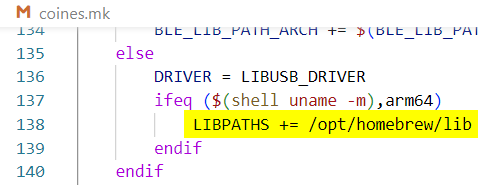
\includegraphics[width=0.6\textwidth]{coinesAPI_images/Mac_libusb_include.png}
            \caption{COINES file structure}
        \end{center}
    \end{figure}
\end{enumerate}

\item \textbf{How do I recover the original program when bootloader was erased accidentally on Application Board 3.x?}
\newline COINES SDK does not provide a way to restore the board to original state.

\item \textbf{How to run multiple application boards using COINES in a single computer?}
\newline When multiple USB devices are connected to a PC, by configuring Serial COM settings for a script, one can communicate with them separately. Please refer to \ref{serialComConfig} for implementation.

\end{enumerate}
For more FAQs, visit \href{https://community.bosch-sensortec.com/t5/MEMS-sensors-forum/bd-p/bst_community-mems-forum}{Bosch Sensortec MEMS sensors forum}.


\newpage
\section{Annexure}
\subsection{GPIO mapping}

\subsubsection{GPIO mapping of APP2.0 shuttle board pins}

The APP2.0 shuttle board has total of 28 pins, of which some have a predefined functionality and some can be used as GPIO by the user.

The shuttle board connector details are given in the table below.

\begin{table}[H]
	\centering
	\begin{tabular}{|c|c|c|c|}
		\hline
		\textbf{Pin number on} & \textbf{Name /} & \textbf{Pin number on} & \textbf{Name /} \\
		\textbf{shuttle board} & \textbf{function} & \textbf{shuttle board} & \textbf{function} \\
		\hline\hline
		1 & VDD (3.3V) & 28 & SHTLE\_COD \#4 \\ \hline
		2 & VDDIO (3.3V) & 27 & SHTLE\_COD \#3 \\ \hline
		3 & GND & 26 & SHTLE\_COD \#2 \\ \hline
		4 & SPI MISO & 25 & SHTLE\_COD \#1 \\ \hline
		5 & SPI: MOSI / I\textsuperscript{2}C: SDA & 24 & SHTLE\_COD \#0 \\ \hline
		6 & SPI: SCK / I\textsuperscript{2}C: SCL & 23 & SHTLE\_COD\_GND \\ \hline
		7 & SPI: CS & 22 & IO\_4 ( GPIO \#4 ) \\ \hline
		8 & IO\_5 ( GPIO \#5 ) & 21 & IO\_7 ( GPIO \#7 ) \\ \hline
		9 & IO\_0 ( GPIO \#0 ) & 20 & IO\_6 ( GPIO \#6 ) \\ \hline 
		10 & SHTLE\_COD \#5 & 19 & IO\_8 ( GPIO \#8 ) \\ \hline 
		11 & SHTLE\_COD \#6 & 18 & SCL (see note) \\ \hline 
		12 & SHTLE\_COD \#7 & 17 & SDA (see note)\\ \hline 
		13 & SHTLE\_COD \#8 & 16 & IO\_3 ( GPIO \#3 ) \\ \hline
		14 & IO\_1 ( GPIO \#1 ) & 15 & IO\_2 ( GPIO \#2 ) \\ \hline
	\end{tabular}
	\caption{Overview of shuttle board pins and their function}
	\label{tab:shtbrdpins}
\end{table}

Note:
\begin{itemize}
	\item In COINES functions, the pins are addressed using the same numbers as on the shuttle board. For example, the GPIO \#5 has the pin number 8.
	\item In some cases (depending on the sensor), the I\textsuperscript{2}C lines are shuttle board pin 6 for the clock signal SCL and shuttle board pin 5 for the data line SDA. In such cases pins 17 and 18 may not be connected. Please carefully read the shuttle board documentation.
\end{itemize}

\subsubsection{GPIO mapping of APP3.x shuttle board pins}

The APP3.x shuttle board has a total of 16 pins, 7 on the left and 9 on the right. (with shuttle board pins facing downwards)

Note:
\begin{itemize}
	\item In COINES functions, the pins are addressed as on the APP3.x shuttle board. For example, the GPIO \#5 is addressed as \texttt{COINES\_MINI\_SHUTTLE\_PIN\_2\_6}.
	\item Supported VDD voltages on APP3.x are 0, 1.8V and 2.8V.
	\item Supported VDDIO voltage on APP3.x is 1.8V.
\end{itemize}

\begin{table}[H]
	\centering
	\begin{tabular}{|c|c|c|c|}
		\hline
		\textbf{Pin number on} & \textbf{Name /} & \textbf{Pin number on} & \textbf{Name /} \\
		\textbf{shuttle board} & \textbf{function} & \textbf{shuttle board} & \textbf{function} \\
		\hline\hline
		1\_1 & VDD (1.8/2.8V) & 2\_1 & SPI\_CS \\ \hline
		1\_2 & VDDIO (1.8) & 2\_2 & SPI: SCK / I\textsuperscript{2}C: SCL \\ \hline
		1\_3 & GND & 2\_3 & SPI: MISO \\ \hline
		1\_4 & GPIO0 & 2\_4 & SPI: MOSI /  I\textsuperscript{2}C: SDA \\ \hline
		1\_5 & GPIO1 & 2\_5 & GPIO4\textsuperscript{*} \\ \hline
		1\_6 & GPIO2 & 2\_6 & GPIO5\textsuperscript{*} \\ \hline
		1\_7 & GPIO3 & 2\_7 & IOXP\_INT\textsuperscript{*}\\ \hline
		     &       & 2\_8 & PlugDet\textsuperscript{*} \\ \hline
		     &       & 2\_9 & EEPROM\_RW \\ \hline
	\end{tabular}
	\caption{Overview of APP3.x shuttle board pins and their function}
	\label{tab:shtbrdpins}
	\textsuperscript{*}SPI pins for secondary interface - CS:GPIO4, SCK:GPIO5, MISO:IOXP\_INT, MOSI:PlugDet
\end{table}

\newpage
\subsection{COINES C functions}\label{CoinesCFunctions}
\subsubsection{coinesAPI calls: Interface and board information}

\paragraph{coines\_open\_comm\_intf}
Opens the communication interface.

\begin{lstlisting}
int16_t coines_open_comm_intf(enum coines_comm_intf intf_type,void *arg); 
\end{lstlisting}

In case of MCU Target, API waits indefinitely for serial port or BLE connection (\texttt{MCU\_APP30} target and \texttt{MCU\_APP31} target).

In case of PC Target, one can configure communication settings either by passing the address of \texttt{coines\_serial\_com\_config} or \texttt{ble\_peripheral\_info} to \texttt{*arg}.

Serial\ com\ configuration:
\newline If \texttt{*arg} is NULL for \texttt{COINES\_COMM\_INTF\_USB}, first com port enumerated will be used for communication.
The serial com configuration structure contains the following items. Refer to \ref{serialComConfig} for its implementation.

\begin{lstlisting}
struct coines_serial_com_config
{
	uint32_t baud_rate; /*< Baud rate */
	uint16_t vendor_id; /*< vendor Id */
	uint16_t product_id; /*< Product Id */
	char* com_port_name; /*< serial com port name */
	uint16_t rx_buffer_size; /*< RX response buffer size */
};
\end{lstlisting}

BLE\ com\ configuration:
\newline If \texttt{*arg} is NULL for \texttt{COINES\_COMM\_INTF\_BLE}, the nearest Application board for the host BLE will be used for communication.
The ble com configuration structure contains the following items. Refer to \ref{bleComConfig} for its implementation.

\begin{lstlisting}
struct ble_peripheral_info
{
	char ble_address[COINES_CHAR_MAX_LEN]; /*< BLE device address */
	char ble_identifier[COINES_CHAR_MAX_LEN]; /*< BLE device identifier */
};
\end{lstlisting}

\paragraph{coines\_close\_comm\_intf}
Closes the communication interface.

\begin{lstlisting}
int16_t coines_close_comm_intf(enum coines_comm_intf intf_type,void *arg); 
\end{lstlisting}

\paragraph{coines\_get\_board\_info}
Gets the board information.

\begin{lstlisting}
int16_t coines_get_board_info(struct coines_board_info *data);
\end{lstlisting}

The data structure contains the following items 

\begin{lstlisting}
struct coines_board_info {
	/*!Board hardware ID */
	uint16_t hardware_id;
	/*!Board software ID */
	uint16_t software_id;
	/*!Type of the board like APP2.0, Arduino Due*/
	uint8_t board;
	/*!Shuttle ID of the sensor connected*/
	uint16_t shuttle_id;
};
\end{lstlisting}

\subsubsection{coinesAPI calls: GPIO oriented calls}

\paragraph{coines\_set\_pin\_config}
Sets the pin direction and the state.

\begin{lstlisting}
int16_t coines_set_pin_config(enum coines_multi_io_pin pin_number, enum coines_pin_direction direction, enum coines_pin_value pin_value);  
\end{lstlisting}

\paragraph{coines\_get\_pin\_config}
Gets the pin configuration.

\begin{lstlisting}
int16_t coines_get_pin_config(enum coines_multi_io_pin pin_number, enum coines_pin_direction *pin_direction, enum coines_pin_value *pin_value);
\end{lstlisting}

\paragraph{coines\_set\_shuttleboard\_vdd\_vddio\_config}
Configures the VDD and VDDIO of the sensor. For APP2.0, a voltage level of 0 or 3300 mV is supported. Any values above 0 will default to 3300 mV.

\begin{lstlisting}
int16_t coines_set_shuttleboard_vdd_vddio_config(uint16_t vdd_millivolt, uint16_t vddio_millivolt);
\end{lstlisting}

\subsubsection{coinesAPI calls: Sensor communication}

\paragraph{coines\_config\_i2c\_bus}
Configures the I\textsuperscript{2}C bus. 

\begin{lstlisting}
int16_t coines_config_i2c_bus(enum coines_i2c_bus bus, enum coines_i2c_mode i2c_mode);
\end{lstlisting}

The first argument refers to the bus on the board. Currently, on APP2.0, there is only one bus available, so the argument is always COINES\_I2C\_BUS\_0.

The following I\textsuperscript{2}C modes are available:
\begin{lstlisting}
COINES_I2C_STANDARD_MODE
COINES_I2C_FAST_MODE
COINES_I2C_SPEED_3_4_MHZ
COINES_I2C_SPEED_1_7_MHZ
\end{lstlisting}

\paragraph{coines\_config\_spi\_bus}
Configures the SPI bus of the board. The argument coines\_spi\_bus refers to the bus on the board. On APP2.0, there is only one bus available, so the user should only use COINES\_SPI\_BUS\_0. The SPI speed can be chosen in various discrete steps, as defined in enum coines\_spi\_speed in coines.h. (For example, COINES\_SPI\_SPEED\_2\_MHZ sets the SPI speed to 2 MHz.)

\begin{lstlisting}
int16_t coines_config_spi_bus(enum coines_spi_bus bus, uint32_t spi_speed, enum coines_spi_mode spi_mode);
\end{lstlisting}

\paragraph{coines\_config\_i2s\_bus}
This API is used to configure the I\textsuperscript{2}S bus to match the TDM configuration

\begin{lstlisting}
int16_t coines_config_i2s_bus(uint16_t data_words, coines_tdm_callback callback);
\end{lstlisting}

Arguments:
\begin{itemize}
	\item \texttt{data\_words}: number of words to use in the buffer. Max is set at COINES\_TDM\_BUFFER\_SIZE\_WORDS.
	\item \texttt{callback}: register a callback to be called to process and copy the data.
\end{itemize}

\paragraph{coines\_deconfig\_spi\_bus}
This API is used to de-configure the SPI bus

\begin{lstlisting}
int16_t coines_deconfig_spi_bus(enum coines_spi_bus bus);
\end{lstlisting}

\paragraph{coines\_deconfig\_i2c\_bus}
This API is used to de-configure the I\textsuperscript{2}C bus

\begin{lstlisting}
int16_t coines_deconfig_i2c_bus(enum coines_i2c_bus bus);
\end{lstlisting}

\paragraph{coines\_deconfig\_i2s\_bus}
This API is used to stop the I\textsuperscript{2}S/TDM interface from reading data from the sensor

\begin{lstlisting}
void coines_deconfig_i2s_bus(void);
\end{lstlisting}

\paragraph{coines\_write\_i2c}\label{CoinesWriteI2c}
Writes 8-bit register data to the I\textsuperscript{2}C device at \texttt{COINES\_I2C\_BUS\_0}.

\begin{lstlisting}
int8_t coines_write_i2c(enum coines_i2c_bus bus,uint8_t dev_addr, uint8_t reg_addr, uint8_t *reg_data, uint16_t count);
\end{lstlisting}

Arguments:
\begin{itemize}
	\item \texttt{bus}: I\textsuperscript{2}C bus to be used
	\item \texttt{dev\_addr}: I\textsuperscript{2}C device address.
	\item \texttt{reg\_addr}: Starting address for writing the data.
	\item \texttt{reg\_data}: Data to be written.
	\item \texttt{count}: Number of bytes to write.
\end{itemize}

\paragraph{coines\_read\_i2c}\label{CoinesReadI2c}
Reads 8-bit register data from the I\textsuperscript{2}C device at \texttt{COINES\_I2C\_BUS\_0}.

\begin{lstlisting}
int8_t coines_read_i2c(enum coines_i2c_bus bus,uint8_t dev_addr, uint8_t reg_addr, uint8_t *reg_data, uint16_t count);
\end{lstlisting}

Arguments:
\begin{itemize}
	\item \texttt{bus}: I\textsuperscript{2}C bus to be used
	\item \texttt{dev\_addr}: I\textsuperscript{2}C device address.
	\item \texttt{reg\_addr}: Starting address for reading the data.
	\item \texttt{reg\_data}: Buffer to take up the read data.
	\item \texttt{count}: Number of bytes to read.
\end{itemize}

\paragraph{coines\_i2c\_set}
This API is used to write the data in I2C communication.

\begin{lstlisting}
int8_t coines_i2c_set(enum coines_i2c_bus bus, uint8_t dev_addr, uint8_t *data, uint8_t count);
\end{lstlisting}

Arguments:
\begin{itemize}
	\item \texttt{bus}: I\textsuperscript{2}C bus to be used
	\item \texttt{dev\_addr}: I\textsuperscript{2}C device address.
	\item \texttt{data}: Data to be written.
	\item \texttt{count}: Number of bytes to write.
\end{itemize}

\paragraph{coines\_i2c\_get}
This API is used to read the data in I2C communication.

\begin{lstlisting}
int8_t coines_i2c_get(enum coines_i2c_bus bus, uint8_t dev_addr, uint8_t *data, uint8_t count);
\end{lstlisting}

Arguments:
\begin{itemize}
	\item \texttt{bus}: I\textsuperscript{2}C bus to be used
	\item \texttt{dev\_addr}: I\textsuperscript{2}C device address.
	\item \texttt{data}: Data read from the sensor.
	\item \texttt{count}: Number of bytes to read.
\end{itemize}

\paragraph{coines\_write\_spi}\label{CoinesWriteSpi}
Writes 8-bit register data to the SPI device at \texttt{COINES\_SPI\_BUS\_0}.

\begin{lstlisting}
int8_t coines_write_spi(enum coines_spi_bus bus,uint8_t dev_addr, uint8_t reg_addr, uint8_t *reg_data, uint16_t count);
\end{lstlisting}

Arguments:
\begin{itemize}
	\item \texttt{bus}: SPI bus to be used.
	\item \texttt{dev\_addr}: Chip select pin number.
	\item \texttt{reg\_addr}: Starting address for writing the data.
	\item \texttt{reg\_data}: Data to be written.
	\item \texttt{count}: Number of bytes to write.
\end{itemize}

\paragraph{coines\_read\_spi}\label{CoinesReadSpi}
Reads 8-bit register data from the SPI device at \texttt{COINES\_SPI\_BUS\_0}.

\begin{lstlisting}
int8_t coines_read_spi(enum coines_spi_bus bus,uint8_t dev_addr, uint8_t reg_addr, uint8_t *reg_data, uint16_t count);
\end{lstlisting}

Arguments:
\begin{itemize}
	\item \texttt{bus}: SPI bus to be used.
	\item \texttt{dev\_addr}: Chip select pin number.
	\item \texttt{reg\_addr}: Starting address for reading the data.
	\item \texttt{reg\_data}: Buffer to take up the read data.
	\item \texttt{count}: Number of bytes to read.
\end{itemize}

\paragraph{coines\_delay\_msec}
Introduces delay in millisecond.

\begin{lstlisting}
void coines_delay_msec(uint32_t delay_ms);
\end{lstlisting}

\paragraph{coines\_delay\_usec}
Introduces delay in microsecond.

\begin{lstlisting}
void coines_delay_usec(uint32_t delay_us);
\end{lstlisting}

\paragraph{coines\_uart\_init}
This API is used to initialize the UART communication

\begin{lstlisting}
int8_t coines_uart_init(enum coines_uart_instance uart_instance, enum coines_uart_parity parity, enum coines_uart_flow_control flow_control, uint32_t baud_rate);
\end{lstlisting}

Arguments:
\begin{itemize}
	\item \texttt{uart\_instance}: Specifies the UART instance
	\item \texttt{parity}: UART parity
	\item \texttt{flow\_control}: UART flow control mode
	\item \texttt{baud\_rate}:  UART baud rate
\end{itemize}

\paragraph{coines\_uart\_read}
This API is used to read the data in UART communication

\begin{lstlisting}
uint16_t coines_uart_read(enum coines_uart_instance uart_instance, uint8_t *buffer, uint16_t length);
\end{lstlisting}

Arguments:
\begin{itemize}
	\item \texttt{uart\_instance}: Specifies the UART instance
	\item \texttt{buffer}: Pointer to the buffer to store the data
	\item \texttt{length}: Length of the buffer
\end{itemize}

\paragraph{coines\_uart\_write}
This API is used to write the data in UART communication

\begin{lstlisting}
int8_t coines_uart_write(enum coines_uart_instance uart_instance, uint8_t *buffer, uint16_t length);
\end{lstlisting}

Arguments:
\begin{itemize}
	\item \texttt{uart\_instance}: Specifies the UART instance
	\item \texttt{buffer}: Pointer to the data buffer which need to be written
	\item \texttt{length}: Length of the buffer
\end{itemize}

\subsubsection{coinesAPI calls: Streaming feature}

Note :
\begin{enumerate}
\item The below APIs are supported only on PC Target.
\item A simpler approach of using \texttt{coines\_attach\_interrupt()} API for is available for MCU.
\end{enumerate}


\paragraph{coines\_config\_streaming}
Sets the configuration for streaming sensor data.

\begin{lstlisting}
int16_t coines_config_streaming(uint8_t channel_id, struct coines_streaming_config *stream_config, struct coines_streaming_blocks *data_blocks); 
\end{lstlisting}

Arguments:
\begin{itemize}
\item \texttt{channel\_id}: An integer number that can be used as identifier/index to the sensor data that will be streamed for this setting

\item \texttt{stream\_config}: Contains information regarding interface settings and streaming configuration.
\item  \texttt{coines\_streaming\_blocks}: Contains information regarding numbers of blocks to read, register address and size for each block.
\end{itemize}
Note:\newline
The below parameters should always be set:
	\begin{itemize}
		\item \texttt{data\_block.no\_of\_blocks}: number of blocks to stream (must at least be one)
		\item For each block b:
		\begin{itemize}
			\item \texttt{data\_block.reg\_start\_addr[b]}: start address of the block in the register map
			\item \texttt{stream\_block.no\_of\_data\_bytes[b]}: number of bytes to read, starting from the start address
		\end{itemize}
	\end{itemize}

For reading data from I\textsuperscript{2}C bus,then set the below parameters:
	
	\begin{itemize}
		\item \texttt{stream\_config.intf = COINES\_SENSOR\_INTF\_I2C;}
		\item \texttt{stream\_config.i2c\_bus}: I\textsuperscript{2}C bus (in case of APP2.0, this is always \texttt{COINES\_I2C\_BUS\_0})
		\item \texttt{stream\_config.dev\_addr}: I\textsuperscript{2}C address of the sensor
	\end{itemize}
For reading data from SPI bus, then set the below parameters:
	\begin{itemize}
		\item \texttt{stream\_config.intf = COINES\_SENSOR\_INTF\_SPI;}
		\item \texttt{stream\_config.spi\_bus}: SPI bus (in case of APP2.0, this is always \texttt{COINES\_SPI\_BUS\_0})
		\item \texttt{stream\_config.cs\_pin}: CS pin of the sensor, information can be obtained from the shuttle board documentation for the sensor. 
	\end{itemize}
When polling mode is requested, set the below parameters:
	\begin{itemize}
		\item \texttt{stream\_config.sampling\_units}: \\ either milliseconds (\texttt{COINES\_SAMPLING\_TIME\_IN\_MILLI\_SEC}) \\ or microseconds (\texttt{COINES\_SAMPLING\_TIME\_IN\_MICRO\_SEC})
		\item \texttt{stream\_config.sampling\_time}: sampling period in the unit as defined in \\ \texttt{stream\_config.sampling\_units}
	\end{itemize}
When interrupt mode is requested, set the below parameters:
	\begin{itemize}
		\item \texttt{stream\_config.int\_pin}: pin of the interrupt which shall trigger the sensor read-out. If the interrupt output of the sensor is used, the required information about the pin number can be obtained from the shuttle board documentation for the sensor.
		\item \texttt{stream\_config.int\_timestamp}:  it can be configured if the sensor data is tagged with a timestamp (\texttt{COINES\_TIMESTAMP\_ENABLE}) or not (\texttt{COINES\_TIMESTAMP\_DISABLE}).
	\end{itemize}

\paragraph{coines\_start\_stop\_streaming}
Starts or stops sensor data streaming.

\begin{lstlisting}
int16_t coines_start_stop_streaming(enum coines_streaming_mode stream_mode, uint8_t start_stop);
\end{lstlisting}

Arguments:
\begin{itemize}
	\item \texttt{stream\_mode}: streaming mode (either \texttt{COINES\_STREAMING\_MODE\_POLLING} or \\ \texttt{COINES\_STREAMING\_MODE\_INTERRUPT})
	\item \texttt{start\_stop}: flag to either start (\texttt{COINES\_STREAMING\_START}) or stop (\texttt{COINES\_STREAMING\_STOP}) the streaming
\end{itemize}

\paragraph{coines\_read\_stream\_sensor\_data}\label{coinesReadStreamSensorData}
Reads the data streamed from the sensor.

\begin{lstlisting}
int16_t coines_read_stream_sensor_data(uint8_t sensor_id, uint32_t number_of_samples, uint8_t *data, uint32_t *valid_samples_count);
\end{lstlisting}

Arguments:
\begin{itemize}
	\item \texttt{sensor\_id}: id of the sensor 
	\item \texttt{number\_of\_samples}: number of samples the user wishes to read (not implemented)
	\item \texttt{data}: data buffer
	\begin{itemize} 
	   \item Interrupt streaming - Packet counter + Register data + Timestamp
	   \item Polling streaming - Register data
	\end{itemize}
	\item \texttt{valid\_samples\_count}: number of samples the user has actually received (may be less than \texttt{number\_of\_samples})
\end{itemize}

Example of a packet:

\begin{figure}[h]
	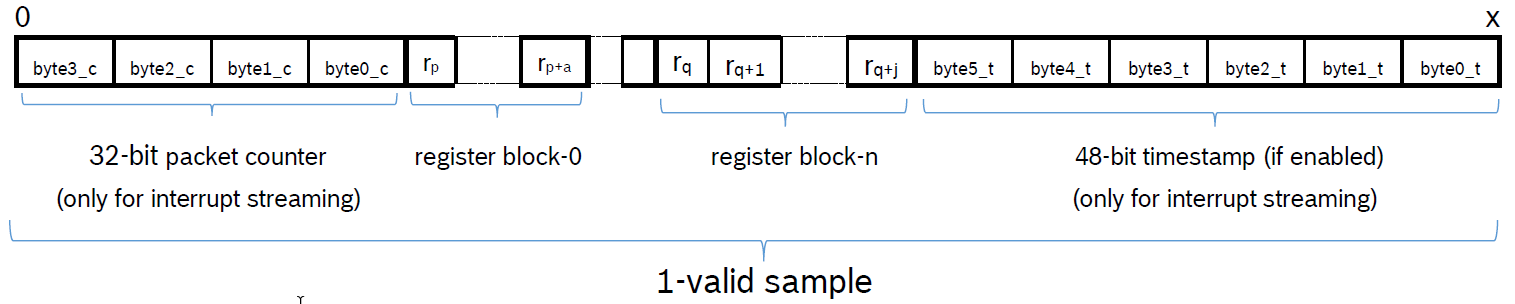
\includegraphics[width=\textwidth]{coinesAPI_images/COINES_streamingSample}
	\caption{Format of streaming packages}
\end{figure}

In the above figure, the following meaning apply to the mentioned abreviations:
\begin{itemize}
	\item r\textsubscript{p}: Value at register address p
	\item a: Size of register block–0
	\item r\textsubscript{p+a}: Value at register address p
\end{itemize}

Similarly is the case for r\textsubscript{q}, j and r\textsubscript{q+j}. See the \texttt{coines\_streaming\_blocks} structure for information regarding register blocks.

The packet counter and the timestamp can be obtained as follows:

\begin{itemize}
	\item[] \texttt{packet\_counter = (byte3\_c << 24) | (byte2\_c << 16) | (byte1\_c << 8) | (byte0\_c)}
	\item[] \texttt{timestamp = (byte5\_t << 40) | (byte4\_t << 32) | (byte3\_t << 24) | (byte2\_t << 16) | (byte1\_t << 8) | (byte0\_t)}
\end{itemize}

The 48-bit timestamp is enabled by using \\ \texttt{coines\_trigger\_timer(COINES\_TIMER\_START,  COINES\_TIMESTAMP\_ENABLE);}

Timestamp in microseconds can be obtained using below formula:
\begin{itemize}
	\item[] $\displaystyle Timestamp\ (\mu s) = \frac{48bit\_timestamp}{30}$
\end{itemize}

\paragraph{coines\_trigger\_timer}
Triggers the timer in firmware and also enables or disables the time stamp feature.

\begin{lstlisting}
int16_t coines_trigger_timer(enum coines_timer_config tmr_cfg,enum coines_time_stamp_config ts_cfg);
\end{lstlisting}

Arguments:
\begin{itemize}
	\item \texttt{tmr\_cfg}: start, stop or reset the timer (\texttt{COINES\_TIMER\_START}, \texttt{COINES\_TIMER\_STOP} or \\ \texttt{COINES\_TIMER\_RESET}) 
	\item \texttt{ts\_cfg}: Enables/disables microcontroller timestamp  (\texttt{COINES\_TIMESTAMP\_ENABLE} or \\ \texttt{COINES\_TIMESTAMP\_DISABLE}) 
\end{itemize}

\subsubsection{coinesAPI calls: Other useful APIs}
\paragraph{coines\_get\_millis}
Returns the number of milliseconds passed since the program started

\begin{lstlisting}
uint32_t coines_get_millis();
\end{lstlisting}

\paragraph{coines\_get\_micro\_sec}
Returns the number of microseconds passed since the program started

\begin{lstlisting}
uint64_t coines_get_micro_sec();
\end{lstlisting}

\paragraph{coines\_attach\_interrupt}
Attaches an interrupt to a Multi-IO pin.Works only on MCU.

\begin{lstlisting}
void coines_attach_interrupt(enum coines_multi_io_pin pin_number,void (*callback)(uint32_t, uint32_t),enum coines_pin_interrupt_mode int_mode);
\end{lstlisting}

Arguments:
\begin{itemize}
	\item \texttt{pin\_number}:  Multi-IO pin
	\item \texttt{callback}: Name of the function to be called on detection of interrupt
	\item \texttt{int\_mode}: Trigger modes - change (\texttt{COINES\_PIN\_INTERRUPT\_CHANGE}), \\
	rising edge (\texttt{COINES\_PIN\_INTERRUPT\_RISING\_EDGE}), \\falling edge (\texttt{COINES\_PIN\_INTERRUPT\_FALLING\_EDGE})
\end{itemize}

\paragraph{coines\_detach\_interrupt}
Detaches interrupt from a Multi-IO pin.Works only on MCU.

\begin{lstlisting}
void coines_detach_interrupt(enum coines_multi_io_pin pin_number);
\end{lstlisting}

Arguments:
\begin{itemize}
	\item \texttt{pin\_number}: Multi-IO pin.
\end{itemize}

\paragraph{coines\_intf\_available}
Return the number of bytes available in the read buffer of the interface.Works only on APP3.x MCU target.

\begin{lstlisting}
uint16_t coines_intf_available(enum coines_comm_intf intf);
\end{lstlisting}

Arguments:
\begin{itemize}
	\item \texttt{intf}: Type of interface (USB, COM, or BLE)
\end{itemize}

\paragraph{coines\_intf\_connected}
Check if the interface is connected.Works only on APP3.x MCU target.

\begin{lstlisting}
bool coines_intf_connected(enum coines_comm_intf intf);
\end{lstlisting}

Arguments:
\begin{itemize}
	\item \texttt{intf}: Type of interface (USB, COM, or BLE)
\end{itemize}

\paragraph{coines\_flush\_intf}
Flush the write buffer.Works only on APP3.x MCU target.

\begin{lstlisting}
void coines_flush_intf(enum coines_comm_intf intf);
\end{lstlisting}

Arguments:
\begin{itemize}
	\item \texttt{intf}: Type of interface (USB, COM, or BLE)
\end{itemize}

\paragraph{coines\_read\_intf}
Read data over the specified interface.Works only on APP3.x MCU target.

\begin{lstlisting}
uint16_t coines_read_intf(enum coines_comm_intf intf, void *buffer, uint16_t len);
\end{lstlisting}

Arguments:
\begin{itemize}
	\item \texttt{intf}: Type of interface (USB, COM, or BLE)
	\item \texttt{buffer}: Pointer to the buffer to store the data
	\item \texttt{len}: Length of the buffer
\end{itemize}

\paragraph{coines\_write\_intf}
Write data over the specified interface.Works only on APP3.x MCU target.

\begin{lstlisting}
uint16_t coines_write_intf(enum coines_comm_intf intf, void *buffer, uint16_t len);
\end{lstlisting}

Arguments:
\begin{itemize}
	\item \texttt{intf}: Type of interface (USB, COM, or BLE)
	\item \texttt{buffer}: Pointer to the buffer storing the data
	\item \texttt{len}: Length of the buffer
\end{itemize}

\paragraph{coines\_get\_version}
Returns pointer to COINES version string

\begin{lstlisting}
char* coines_get_version(void);
\end{lstlisting}

\paragraph{coines\_soft\_reset}
Resets the device. After reset device jumps to the address specified in makefile(APP\_START\_ADDRESS).

\begin{lstlisting}
void coines_soft_reset(void);
\end{lstlisting}

\paragraph{coines\_read\_temp\_data}
This API is used to read the temperature sensor data.

\begin{lstlisting}
int16_t coines_read_temp_data(float *temp_data);
\end{lstlisting}
        
Arguments:
\begin{itemize}
	\item \texttt{temp\_conv\_data}: Buffer to retrieve the sensor data in degree Celsius.
\end{itemize}

\paragraph{coines\_read\_bat\_status}
This API is used to read the battery status.

\begin{lstlisting}
int16_t coines_read_bat_status(uint16_t *bat_status_mv, uint8_t *bat_status_percent);
\end{lstlisting}

Arguments:
\begin{itemize}
	\item \texttt{bat\_status\_mv}: Buffer to retrieve the battery status in millivolt
	\item \texttt{bat\_status\_percent}: Buffer to retrieve the battery status in percentage
\end{itemize}

\paragraph{coines\_ble\_config}
This API is used to configure BLE name and power. It should be called before calling coines\_open\_comm\_intf API.

\begin{lstlisting}
int16_t coines_ble_config(struct coines_ble_config *ble_config);
\end{lstlisting}

Arguments:
\begin{itemize}
	\item \texttt{ble\_config}: structure holding ble name and power details
\end{itemize}

\paragraph{coines\_set\_led}
 This API is used to set led state(on or off).
 
\begin{lstlisting}
int16_t coines_set_led(enum coines_led led,enum coines_led_state led_state);
\end{lstlisting}

Arguments:
\begin{itemize}
	\item \texttt{led}: led to which the state has to be set.
	\item \texttt{led\_state}: state to be set to the given led.
\end{itemize}

\paragraph{coines\_timer\_config}
 This API is used to configure the hardware timer.
 
\begin{lstlisting}
int16_t coines_timer_config(enum coines_timer_instance instance, void* handler);
\end{lstlisting}

Arguments:
\begin{itemize}
	\item \texttt{instance}: timer instance.
	\item \texttt{handler}: callback to be called when timer expires.
\end{itemize}

\paragraph{coines\_timer\_deconfig}
 This API is used to de-configure the hardware timer.
 
\begin{lstlisting}
int16_t coines_timer_deconfig(enum coines_timer_instance instance);
\end{lstlisting}

Arguments:
\begin{itemize}
	\item \texttt{instance}: timer instance.
\end{itemize}

\paragraph{coines\_timer\_start}
 This API is used to start the configured hardware timer.
 
\begin{lstlisting}
int16_t coines_timer_start(enum coines_timer_instance instance, uint32_t timeout);
\end{lstlisting}

Arguments:
\begin{itemize}
	\item \texttt{instance}: timer instance.
	\item \texttt{timeout}: timeout in microseconds.
\end{itemize}

\paragraph{coines\_timer\_stop}
 This API is used to stop the  hardware timer.
 
\begin{lstlisting}
int16_t coines_timer_stop(enum coines_timer_instance instance);
\end{lstlisting}

Arguments:
\begin{itemize}
	\item \texttt{instance}: timer instance.
\end{itemize}

\paragraph{coines\_get\_realtime\_usec}
This API is used to get the current counter(RTC) reference time in usec

\begin{lstlisting}
uint32_t coines_get_realtime_usec(void);
\end{lstlisting}

\paragraph{coines\_delay\_realtime\_usec}
This API is used to introduce delay based on high precision RTC(LFCLK crystal) with the resolution of 30.517 usec.

\begin{lstlisting}
void coines_delay_realtime_usec(uint32_t period);
\end{lstlisting}

Arguments:
\begin{itemize}
	\item \texttt{period}: required delay in microseconds 
\end{itemize}

\paragraph{coines\_attach\_timed\_interrupt}
Attaches a timed interrupt to a Multi-IO pin.

\begin{lstlisting}
int16_t coines_attach_timed_interrupt(enum coines_multi_io_pin pin_number, void (*timed_interrupt_cb)(uint64_t,uint32_t,uint32_t), enum coines_pin_interrupt_mode int_mode);
\end{lstlisting}

Arguments:
\begin{itemize}
	\item \texttt{pin\_number}: Multi-IO pin.
	\item \texttt{timed\_interrupt\_cb}: Name of the function to be called on detection of interrupt.
	\item \texttt{int\_mode}: Trigger modes - change,rising edge,falling edge.
\end{itemize}

\paragraph{coines\_detach\_timed\_interrupt}
Detaches a timed interrupt from a Multi-IO pin.

\begin{lstlisting}
int16_t coines_detach_timed_interrupt(enum coines_multi_io_pin pin_number);
\end{lstlisting}

Arguments:
\begin{itemize}
	\item \texttt{pin\_number}: Multi-IO pin.
\end{itemize}

\paragraph{coines\_echo\_test}
This API is used to test the communication.

\begin{lstlisting}
int16_t coines_echo_test(uint8_t *data, uint16_t length);
\end{lstlisting}

Arguments:
\begin{itemize}
	\item \texttt{data}: Data to be sent for testing.
	\item \texttt{length}: Length of the data.
\end{itemize}

\paragraph{coines\_shuttle\_eeprom\_write}
This API is used to write the content into shuttle eeprom.

\begin{lstlisting}
int16_t coines_shuttle_eeprom_write(uint16_t start_addr, uint8_t *buffer, uint16_t length);
\end{lstlisting}

Arguments:
\begin{itemize}
	\item \texttt{start\_addr}: EEPROM write address.
	\item \texttt{buffer}: Pointer to the buffer.
	\item \texttt{length}: Length of the buffer.
\end{itemize}

\paragraph{coines\_shuttle\_eeprom\_read}
This API is used to read the content from shuttle eeprom.

\begin{lstlisting}
int16_t coines_shuttle_eeprom_read(uint16_t start_addr, uint8_t *buffer, uint16_t length);
\end{lstlisting}

Arguments:
\begin{itemize}
	\item \texttt{start\_addr}: EEPROM read address.
	\item \texttt{buffer}: Pointer to the buffer.
	\item \texttt{length}: Length of the buffer.
\end{itemize}

\paragraph{coines\_yield}
This API can be defined to perform a task when yielded from an ongoing blocking call.

\begin{lstlisting}
void coines_yield(void);
\end{lstlisting}

\paragraph{coines\_execute\_critical\_region}
This API is used to execute the function inside critical region.

\begin{lstlisting}
void coines_execute_critical_region(coines_critical_callback callback);
\end{lstlisting}

Arguments:
\begin{itemize}
	\item \texttt{callback}: function to execute.
\end{itemize}

\paragraph{coines\_scan\_ble\_devices}\label{coinesScanBleDevices}
This API is used to connect to BLE Adapter and return list of BLE peripherals found during BLE scan.

\begin{lstlisting}
	int16_t coines_scan_ble_devices(struct ble_peripheral_info *ble_info, uint8_t *peripheral_count, size_t scan_timeout_ms)
\end{lstlisting}

Arguments:
\begin{itemize}
	\item \texttt{ble\_info}: array of struct containing found BLE peripheral information
	\item \texttt{peripheral\_count}: number of BLE peripherals found
	\item \texttt{scan\_timeout\_ms}: timeout for BLE scan
\end{itemize}

\newpage


\newpage
\subsection{COINES Python functions}

As coinespy is only a wrapper on top of coinesAPI, the following API documentation is limited to the wrapper only. Details about meaning of variables and functionality can be found in the corresponding coinesAPI documentation in the chapter above.
\vspace{12pt}
The following function calls are defined within the class \texttt{CoinesBoard}. Thus in order to access the functions, the user has to create an object of that class first.

\begin{lstlisting}[language=python]
	import coinespy as cpy
	coinesboard = cpy.CoinesBoard()
\end{lstlisting}

\subsubsection{coinespy API calls: Interface and board information}

\paragraph{open\_comm\_interface}
Sets the communication interface between board and PC to USB, Serial or BLE.

\begin{lstlisting}[language=python]
coinesboard.open_comm_interface(interface=CommInterface.USB, serial_com_config: SerialComConfig = None,
ble_com_config: BleComConfig = None) -> ErrorCodes
\end{lstlisting}

For the definition of \texttt{CommInterface}, refer to \ref{CommInterface}.

\paragraph{close\_comm\_interface}
Disposes the resources used by the USB/serial/BLE communication.

\begin{lstlisting}[language=python]
coinesboard.close_comm_interface(arg=None) -> ErrorCodes
\end{lstlisting}

\paragraph{get\_board\_info}
Obtains board specific information.

\begin{lstlisting}[language=python]
BoardInfo = coinesboard.get_board_info()

# Return:
BoardInfo.HardwareId    # Hardware ID
BoardInfo.SoftwareId    # Firmware version information
BoardInfo.Board         # Board type
BoardInfo.ShuttleID     # ID of shuttle, in case a shuttle is detected
\end{lstlisting}

\paragraph{scan\_ble\_devices}
This API is used to connect to BLE Adapter and return list of BLE peripherals found during BLE scan.

\begin{lstlisting}
ble_info, peripheral_count  = coinesboard.scan_ble_devices(scan_timeout_ms=0) -> Tuple[list, int]
\end{lstlisting}

For the definition of parameters, refer to \ref{coinesScanBleDevices}.

\paragraph{echo\_test}
This API is used to test the communication.

\begin{lstlisting}
coinesboard.echo_test(data: List[int]) -> ErrorCodes
\end{lstlisting}

Arguments:
\begin{itemize}
	\item \texttt{data}: Data to be sent for testing.
\end{itemize}

\subsubsection{coinespy API calls: GPIO oriented calls}

\paragraph{set\_pin\_config}
Configures the state, level and direction of a GPIO pin

\begin{lstlisting}[language=python]
coinesboard.set_pin_config(pin_number: MultiIOPin, direction: PinDirection, output_state: PinValue) -> ErrorCodes
\end{lstlisting}

For the definition of \texttt{MultiIOPin}, refer to \ref{MultiIOPin}. For the definition of \texttt{PinDirection}, refer to \ref{PinDirection}.
For \texttt{PinValue}, refer to \ref{PinValue}.

\paragraph{get\_pin\_config}
Obtains information regarding the Pin's state, level and direction.

\begin{lstlisting}[language=python]
PinConfigInfo = coinesboard.get_pin_config(pin_number: MultiIOPin)

# Return:
PinConfigInfo.direction         # 0: INPUT, 1: OUTPUT
PinConfigInfo.switch_state       # 0: OFF, 1: ON
PinConfigInfo.level             # 1: HIGH, 0: LOW
\end{lstlisting}

\paragraph{set\_shuttleboard\_vdd\_vddio\_config}

Set the VDD and VDDIO voltage level.

\begin{lstlisting}
coinesboard.set_shuttleboard_vdd_vddio_config(vdd_val: float = None, vddio_val: float = None) -> ErrorCodes

# Example: coinesboard.set_shuttleboard_vdd_vddio_config(3.3, 3.3)
\end{lstlisting}

\paragraph{set\_vdd}

Set the VDD voltage level.

\begin{lstlisting}
coinesboard.set_vdd(vdd_val: float = None) -> ErrorCodes

# Example: coinesboard.set_vdd(3.3)
\end{lstlisting}

\paragraph{set\_vddio}

Set the VDDIO voltage level.

\begin{lstlisting}
coinesboard.set_vddio(vdd_val: float = None) -> ErrorCodes

# Example: coinesboard.set_vddio(3.3)
\end{lstlisting}

\subsubsection{coinespy API calls: Sensor communication}

For the definition of \texttt{SPIBus}, refer to \ref{SPIBus}. For the definition of \texttt{I2CBus}, refer to \ref{I2CBus}.

\paragraph{config\_i2c\_bus}
Configures the I\textsuperscript{2}C bus.

\begin{lstlisting}
coinesboard.config_i2c_bus(bus: I2CBus, i2c_address: int, i2c_mode: I2CMode) -> ErrorCodes
\end{lstlisting}

For the definition of \texttt{I2CMode}, refer to \ref{I2CMode}.

\paragraph{config\_spi\_bus}
Configures the SPI bus of the board.
\begin{lstlisting}
coinesboard.config_spi_bus(bus: SPIBus, cs_pin: MultiIOPin, spi_speed=SPISpeed, spi_mode=SPIMode) -> ErrorCodes
\end{lstlisting}

For the definition of \texttt{MultiIOPin}, refer to \ref{MultiIOPin}. For the definition of \texttt{SPISpeed}, refer to \ref{SPISpeed}. For the definition of \texttt{SPIMode}, refer to \ref{SPIMode}.

\paragraph{deconfig\_i2c\_bus}
This API is used to de-configure the I\textsuperscript{2}C bus

\begin{lstlisting}
coinesboard.deconfig_i2c_bus(bus: I2CBus) -> ErrorCodes
\end{lstlisting}

\paragraph{deconfig\_spi\_bus}
This API is used to de-configure the SPI bus

\begin{lstlisting}
coinesboard.deconfig_spi_bus(bus: SPIBus) -> ErrorCodes
\end{lstlisting}

\paragraph{write\_i2c}
Writes 8-bit register data to the I\textsuperscript{2}C

\begin{lstlisting}
coinesboard.write_i2c(bus: I2CBus, register_address: int, register_value: int, sensor_interface_detail: int = None) -> ErrorCodes
\end{lstlisting}

For the definition of parameters, refer to \ref{CoinesWriteI2c}.

\paragraph{read\_i2c}
Reads 8-bit register data from the I\textsuperscript{2}C

\begin{lstlisting}
register_data = coinesboard.read_i2c(bus: I2CBus, register_address: int, number_of_reads=1, sensor_interface_detail: int = None)
\end{lstlisting}

For the definition of parameters, refer to \ref{CoinesReadI2c}.

\paragraph{write\_spi}
Writes 8-bit register data to the SPI device

\begin{lstlisting}
coinesboard.write_spi(bus: SPIBus, register_address: int, register_value: int, sensor_interface_detail: int = None) -> ErrorCodes
\end{lstlisting}


For the definition of parameters, refer to \ref{CoinesWriteSpi}.

\paragraph{read\_spi}
Reads 8-bit register data from the SPI device.

\begin{lstlisting}
register_data = coinesboard.read_spi(bus: SPIBus, register_address: int, number_of_reads=1, sensor_interface_detail: int = None)
\end{lstlisting}

For the definition of parameters, refer to \ref{CoinesReadSpi}.

\paragraph{delay\_milli\_sec}
Introduces delay in millisecond.

\begin{lstlisting}
coinesboard.delay_milli_sec(time_in_milli_sec=100)
\end{lstlisting}

\paragraph{delay\_micro\_sec}
Introduces delay in microsecond.

\begin{lstlisting}
coinesboard.delay_micro_sec(time_in_micro_sec=1)
\end{lstlisting}

\subsubsection{coinespy API calls: Streaming feature}

\paragraph{config\_streaming}

Sets the configuration for streaming sensor data.

\begin{lstlisting}[language=python]
coinesboard.config_streaming(sensor_id: int,
	stream_config: StreamingConfig, data_blocks: StreamingBlocks) -> ErrorCodes
\end{lstlisting}

Arguments:
\begin{itemize}
	\item \texttt{sensor\_id}: An integer number that can be used as identifier/index to the sensor data that will be streamed for this setting

	\item \texttt{stream\_config}: Contains information regarding interface settings and streaming configuration.
	\item  \texttt{data\_blocks}: Contains information regarding numbers of blocks to read, register address and size for each block.
\end{itemize}
Note:\newline
The below parameters should always be set:
\begin{itemize}
	\item \texttt{data\_blocks.NoOfBlocks}: number of blocks to stream (must at least be one)
	\item For each block b:
	      \begin{itemize}
		      \item \texttt{data\_blocks.RegStartAddr[b]}: start address of the block in the register map
		      \item \texttt{data\_blocks.NoOfDataBytes[b]}: number of bytes to read, starting from the start address
	      \end{itemize}
\end{itemize}
\vspace{12pt}
For reading data from I\textsuperscript{2}C bus,then set the below parameters:
\begin{itemize}
	\item \texttt{stream\_config.Intf = cpy.SensorInterface.I2C.value}
	\item \texttt{stream\_config.I2CBus}: I\textsuperscript{2}C bus (in case of APP2.0 and APP3.x, this is always\\
	      \texttt{cpy.I2CBus.BUS\_I2C\_0.value})
	\item \texttt{stream\_config.DevAddr}: I\textsuperscript{2}C address of the sensor
\end{itemize}
\vspace{12pt}
For reading data from SPI bus, then set the below parameters:
\begin{itemize}
	\item \texttt{stream\_config.Intf = cpy.SensorInterface.SPI.value;}
	\item \texttt{stream\_config.SPIBus}: SPI bus (in case of APP2.0 and APP3.x, this is always\\
	      \texttt{cpy.SPIBus.BUS\_SPI\_0.value})
	\item \texttt{stream\_config.CSPin}: CS pin of the sensor, information can be obtained from the shuttle board documentation for the sensor.
	\item \texttt{stream\_config.SPIType}: 0 : 8-bit SPI; 1 : 16-bit SPI
\end{itemize}
\vspace{12pt}
When polling mode is requested, set the below parameters:
\begin{itemize}
	\item \texttt{stream\_config.SamplingUnits}: either milliseconds or microseconds. Refer to \ref{SamplingUnits}.
	\item \texttt{stream\_config.SamplingTime}: sampling period in the unit as defined in \\ \texttt{stream\_config.SamplingUnits}
\end{itemize}
\vspace{12pt}
When interrupt mode is requested, set the below parameters:
\begin{itemize}
	\item \texttt{stream\_config.IntPin}: pin of the interrupt which shall trigger the sensor read-out. If the interrupt output of the sensor is used, the required information about the pin number can be obtained from the shuttle board documentation for the sensor.
	\item \texttt{stream\_config.IntTimeStamp}:  it can be configured if the sensor data is tagged with a timestamp - 1 or not - 0.
	\item \texttt{stream\_config.HwPinState}: State of the hardware pin connected to the interrupt line - 0/1 : Low/high
\end{itemize}
\vspace{12pt}
Below parameters are common for both streaming types:
\begin{itemize}
	\item \texttt{stream\_config.IntlineCount}: Number of interrupt lines to be used for monitoring interrupts.
	\item \texttt{stream\_config.IntlineInfo}: List of pin numbers that correspond to interrupt lines being used for interrupt monitoring.
	\item \texttt{stream\_config.ClearOnWrite}: 0/1 : Disable/enable "clear on write" feature
\end{itemize}
\vspace{12pt}
The below parameters should be set only when stream\_config.ClearOnWrite = 1:
\begin{itemize}
	\item \texttt{stream\_config.ClearOnWriteConfig.StartAddress}: Address of the sensor register at which the process of clearOnWrite should initiate.
	\item \texttt{stream\_config.ClearOnWriteConfig.DummyByte}: Number of padding bytes that must be added before clearing the bytes starting from the designated address.
	\item \texttt{stream\_config.ClearOnWriteConfig.NumBytesToClear}: Number of bytes that need to be cleared.
\end{itemize}
\vspace{12pt}
Below is the Python code snippet for interrupt streaming
\begin{lstlisting}[language=Python]
# Store streaming settings in local variables
accel_stream_settings = dict(
	I2C_ADDR_PRIMARY=0x18,
	NO_OF_BLOCKS = 2,
	REG_X_LSB= [0x12, 0x00],
	NO_OF_DATA_BYTES= [6, 1],
	CHANNEL_ID=1,
	CS_PIN=cpy.MultiIOPin.SHUTTLE_PIN_8.value,
	INT_PIN=cpy.MultiIOPin.SHUTTLE_PIN_21.value,
	INT_TIME_STAMP=1,
)
gyro_stream_settings = dict(
	I2C_ADDR_PRIMARY=0x68,
	NO_OF_BLOCKS = 2,
	REG_X_LSB= [0x02,0x00],
	NO_OF_DATA_BYTES = [6, 1],
	CHANNEL_ID=2,
	CS_PIN=cpy.MultiIOPin.SHUTTLE_PIN_14.value,
	INT_PIN=cpy.MultiIOPin.SHUTTLE_PIN_22.value,
	INT_TIME_STAMP=1,
)


# set the config_streaming parameters
stream_config = cpy.StreamingConfig()
data_blocks = cpy.StreamingBlocks()
if self.interface == cpy.SensorInterface.I2C:
	stream_config.Intf = cpy.SensorInterface.I2C.value
	stream_config.I2CBus = cpy.I2CBus.BUS_I2C_0.value
	stream_config.DevAddr = sensor["I2C_ADDR_PRIMARY"]

elif self.interface == cpy.SensorInterface.SPI:
	stream_config.Intf = cpy.SensorInterface.SPI.value
	stream_config.SPIBus = cpy.SPIBus.BUS_SPI_0.value
	stream_config.CSPin = sensor["CS_PIN"]

if sensor_type == bmi08x.SensorType.ACCEL and self.interface == cpy.SensorInterface.SPI:
	# extra dummy byte for SPI
	dummy_byte_offset = 1
else:
	dummy_byte_offset = 0

data_blocks.NoOfBlocks = sensor["NO_OF_BLOCKS"]
for i in range(0, data_blocks.NoOfBlocks):
	data_blocks.RegStartAddr[i] = sensor["REG_X_LSB"][i]
	data_blocks.NoOfDataBytes[i] = sensor["NO_OF_DATA_BYTES"][i] + dummy_byte_offset

stream_config.IntTimeStamp = sensor["INT_TIME_STAMP"]
stream_config.IntPin = sensor["INT_PIN"]

# call config_streaming API for each sensor to configure the streaming settings
ret = coinesboard.config_streaming(
	accel_sensor_id, self.accel_stream_config, self.accel_data_blocks)
ret = coinesboard.config_streaming(
	gyro_sensor_id, self.accel_stream_config, self.accel_data_blocks)

\end{lstlisting}



\paragraph{start\_stop\_streaming}

Starts or stops sensor data streaming.

\begin{lstlisting}[language=python]
coinesboard.start_stop_streaming(stream_mode: StreamingMode, start_stop: StreamingState) -> ErrorCodes
\end{lstlisting}

For the definition of \texttt{StreamingMode}, refer to \ref{StreamingMode}. For the definition of \texttt{StreamingState}, refer to \ref{StreamingState}.

\paragraph{read\_stream\_sensor\_data}

Reads the data streamed from the sensor.

\begin{lstlisting}[language=python]
coinesboard.read_stream_sensor_data(sensor_id: int, number_of_samples: int,
	buffer_size=STREAM_RSP_BUF_SIZE) -> Tuple[ErrorCodes, list, int]
\end{lstlisting}

Return:\\
Tuple of ErrorCodes, data and valid\_samples\_count\newline
For the detailed definition of parameters, refer to \ref{coinesReadStreamSensorData}.

\subsubsection{coinespy API calls: Other useful APIs}

\paragraph{flush\_interface}
Flush the write buffer.

\begin{lstlisting}
coinesboard.flush_interface()
\end{lstlisting}

\paragraph{soft\_reset}
Resets the device.

\begin{lstlisting}
coinesboard.soft_reset()
\end{lstlisting}

\subsubsection{Definition of constants}

\paragraph{PinDirection}\label{PinDirection}

Pin mode definitions

\begin{lstlisting}
class PinDirection:
    INPUT = 0  # COINES_PIN_DIRECTION_IN = 0
    OUTPUT = 1
\end{lstlisting}

\paragraph{PinValue}\label{PinValue}

Pin level definitions

\begin{lstlisting}
class PinValue:
    LOW = 0  # COINES_PIN_VALUE_LOW = 0
    HIGH = 1
\end{lstlisting}

\paragraph{CommInterface}\label{CommInterface}

Definition of Communication interface

\begin{lstlisting}
class CommInterface:
    USB = 0
    SERIAL = 1
    BLE = 2
\end{lstlisting}

\paragraph{I2CMode}\label{I2CMode}

Definition of the speed of I2C bus.

\begin{lstlisting}
class I2CMode:
	STANDARD_MODE = 0 # Standard mode - 100kHz
	FAST_MODE = 1 # Fast mode - 400kHz
	SPEED_3_4_MHZ = 2 # High Speed mode - 3.4 MHz
	SPEED_1_7_MHZ = 3 # High Speed mode 2 - 1.7 MHz
\end{lstlisting}

\paragraph{SPISpeed}\label{SPISpeed}

Definition of the speed of SPI bus.

\begin{lstlisting}
class SPISpeed:
	SPI_10_MHZ = 6
	SPI_7_5_MHZ = 8
	SPI_6_MHZ = 10
	SPI_5_MHZ = 12
	SPI_3_75_MHZ = 16
	SPI_3_MHZ = 20
	SPI_2_5_MHZ = 24
	SPI_2_MHZ = 30
	SPI_1_5_MHZ = 40
	SPI_1_25_MHZ = 48
	SPI_1_2_MHZ = 50
	SPI_1_MHZ = 60
	SPI_750_KHZ = 80
	SPI_600_KHZ = 100
	SPI_500_KHZ = 120
	SPI_400_KHZ = 150
	SPI_300_KHZ = 200
	SPI_250_KHZ = 240
\end{lstlisting}

\paragraph{SPITransferBits}\label{SPITransferBits}

Definition of the SPI bits.

\begin{lstlisting}
class SPITransferBits:
	SPI8BIT = 8 # 8 bit register read/write
	SPI16BIT = 16 # 16 bit register read/write
\end{lstlisting}

\paragraph{SPIMode}\label{SPIMode}

Definition of the SPI mode.

\begin{lstlisting}
class SPIMode:
	MODE0 = 0x00 # SPI Mode 0: CPOL=0; CPHA=0
	MODE1 = 0x01 # SPI Mode 1: CPOL=0; CPHA=1
	MODE2 = 0x02 # SPI Mode 2: CPOL=1; CPHA=0
	MODE3 = 0x03 # SPI Mode 3: CPOL=1; CPHA=1
\end{lstlisting}

\paragraph{MultiIOPin}\label{MultiIOPin}

Definition of the shuttle board pin(s)

\begin{lstlisting}
class MultiIOPin(Enum):
	SHUTTLE_PIN_7 = 0x09 # CS pin
	SHUTTLE_PIN_8 = 0x05 # Multi-IO 5
	SHUTTLE_PIN_9 = 0x00 # Multi-IO 0
	SHUTTLE_PIN_14 = 0x01 # Multi-IO 1
	SHUTTLE_PIN_15 = 0x02 # Multi-IO 2
	SHUTTLE_PIN_16 = 0x03 # Multi-IO 3
	SHUTTLE_PIN_19 = 0x08 # Multi-IO 8
	SHUTTLE_PIN_20 = 0x06 # Multi-IO 6
	SHUTTLE_PIN_21 = 0x07 # Multi-IO 7
	SHUTTLE_PIN_22 = 0x04 # Multi-IO 4
	SHUTTLE_PIN_SDO = 0x1F

	# APP3.x pins
	MINI_SHUTTLE_PIN_1_4 = 0x10  # GPIO0
	MINI_SHUTTLE_PIN_1_5 = 0x11  # GPIO1
	MINI_SHUTTLE_PIN_1_6 = 0x12  # GPIO2/INT1
	MINI_SHUTTLE_PIN_1_7 = 0x13  # GPIO3/INT2
	MINI_SHUTTLE_PIN_2_5 = 0x14  # GPIO4
	MINI_SHUTTLE_PIN_2_6 = 0x15  # GPIO5
	MINI_SHUTTLE_PIN_2_1 = 0x16  # CS
	MINI_SHUTTLE_PIN_2_3 = 0x17  # SDO
	MINI_SHUTTLE_PIN_2_7 = 0x1D  # GPIO6
	MINI_SHUTTLE_PIN_2_8 = 0x1E  # GPIO7
\end{lstlisting}

\paragraph{SensorInterface}\label{SensorInterface}

To define Sensor interface.

\begin{lstlisting}
class SensorInterface(Enum):
	SPI = 0
	I2C = 1
\end{lstlisting}

\paragraph{I2CBus}\label{I2CBus}

Used to define the I2C type.

\begin{lstlisting}
	class I2CBus(Enum):
	BUS_I2C_0 = 0
	BUS_I2C_1 = 1
	BUS_I2C_MAX = 2
\end{lstlisting}

\paragraph{SPIBus}\label{SPIBus}

Used to define the SPI type.

\begin{lstlisting}
	class SPIBus(Enum):
	BUS_SPI_0 = 0
	BUS_SPI_1 = 1
	BUS_SPI_MAX = 2
\end{lstlisting}

\paragraph{PinInterruptMode}\label{PinInterruptMode}

Defines Pin interrupt modes.

\begin{lstlisting}
class PinInterruptMode(Enum):
	# Trigger interrupt on pin state change
	PIN_INTERRUPT_CHANGE = 0
	# Trigger interrupt when pin changes from low to high
	PIN_INTERRUPT_RISING_EDGE = 1
	# Trigger interrupt when pin changes from high to low
	PIN_INTERRUPT_FALLING_EDGE = 2
	PIN_INTERRUPT_MODE_MAXIMUM = 4
\end{lstlisting}

\paragraph{StreamingMode}\label{StreamingMode}

Streaming mode definitions

\begin{lstlisting}
class StreamingMode:
    STREAMING_MODE_POLLING = 0    # Polling mode streaming
    STREAMING_MODE_INTERRUPT = 1  # Interrupt mode streaming
\end{lstlisting}

\paragraph{StreamingState}\label{StreamingState}

Streaming state definitions

\begin{lstlisting}
class StreamingState:
	STREAMING_START = 1
	STREAMING_STOP = 0
\end{lstlisting}

\paragraph{SamplingUnits}\label{SamplingUnits}

Sampling Unit definitions

\begin{lstlisting}
class SamplingUnits:
    SAMPLING_TIME_IN_MICRO_SEC = 0x01  # sampling unit in micro second
    SAMPLING_TIME_IN_MILLI_SEC = 0x02  # sampling unit in milli second
\end{lstlisting}



\newpage
\subsection{Error Codes}

Error codes are not (always) returned by the different function calls. Internally, a \texttt{error\_code} variable is maintained which is updated after the function call. It can be read out and checked by the user afterwards.

C Example
\begin{lstlisting}[language=c]
#include <stdio.h>
#include <stdlib.h>

#include "coines.h"

int main(void)
{
    int16_t error_code = coines_open_comm_intf(COINES_COMM_INTF_USB, NULL);
    if (error_code != COINES_SUCCESS)
    {
        const char *err_str = get_coines_error_str(error_code);
        printf("\n%s", err_str);
        exit(error_code);
    }

    coines_close_comm_intf(COINES_COMM_INTF_USB, NULL);
    return 0;
}
\end{lstlisting}

Python Example
\begin{lstlisting}[language=python]
import coinespy as cpy
board = cpy.CoinesBoard()
try:
	board.open_comm_interface(cpy.CommInterface.USB)
	board.close_comm_interface()
except:
	print(f'Could not connect to board: {board.error_code}')
	exit(board.error_code)
\end{lstlisting}

Error code definitions
\begin{lstlisting}
    COINES_SUCCESS = 0
    COINES_E_FAILURE = -1
    COINES_E_COMM_IO_ERROR = -2
    COINES_E_COMM_INIT_FAILED = -3
    COINES_E_UNABLE_OPEN_DEVICE = -4
    COINES_E_DEVICE_NOT_FOUND = -5
    COINES_E_UNABLE_CLAIM_INTERFACE = -6
    COINES_E_MEMORY_ALLOCATION = -7
    COINES_E_NOT_SUPPORTED = -8
    COINES_E_NULL_PTR = -9
    COINES_E_COMM_WRONG_RESPONSE = -10
    COINES_E_SPI16BIT_NOT_CONFIGURED = -11
    COINES_E_SPI_INVALID_BUS_INTERFACE = -12
    COINES_E_SPI_CONFIG_EXIST = -13
    COINES_E_SPI_BUS_NOT_ENABLED = -14
    COINES_E_SPI_CONFIG_FAILED = -15
    COINES_E_I2C_INVALID_BUS_INTERFACE = -16
    COINES_E_I2C_BUS_NOT_ENABLED = -17
    COINES_E_I2C_CONFIG_FAILED = -18
    COINES_E_I2C_CONFIG_EXIST = -19
    COINES_E_TIMER_INIT_FAILED = -20
    COINES_E_TIMER_INVALID_INSTANCE = -21
    COINES_E_TIMER_CC_CHANNEL_NOT_AVAILABLE = -22
    COINES_E_EEPROM_RESET_FAILED = -23
    COINES_E_EEPROM_READ_FAILED = -24
    COINES_E_INIT_FAILED = -25
    COINES_E_STREAM_NOT_CONFIGURED = -26
    COINES_E_STREAM_INVALID_BLOCK_SIZE = -27
    COINES_E_STREAM_SENSOR_ALREADY_CONFIGURED = -28
    COINES_E_STREAM_CONFIG_MEMORY_FULL = -29
    COINES_E_INVALID_PAYLOAD_LEN = -30
    COINES_E_CHANNEL_ALLOCATION_FAILED = -31
    COINES_E_CHANNEL_DE_ALLOCATION_FAILED = -32
    COINES_E_CHANNEL_ASSIGN_FAILED = -33
    COINES_E_CHANNEL_ENABLE_FAILED = -34
    COINES_E_CHANNEL_DISABLE_FAILED = -35
    COINES_E_INVALID_PIN_NUMBER = -36
    COINES_E_MAX_SENSOR_COUNT_REACHED = -37
    COINES_E_EEPROM_WRITE_FAILED = -38
    COINES_E_INVALID_EEPROM_RW_LENGTH = -39
    COINES_E_INVALID_SCOM_CONFIG = -40
    COINES_E_INVALID_BLE_CONFIG = -41
    COINES_E_SCOM_PORT_IN_USE = -42
    COINES_E_UART_INIT_FAILED = -43
    COINES_E_UART_WRITE_FAILED = -44
    COINES_E_UART_INSTANCE_NOT_SUPPORT = -45
    COINES_E_BLE_ADAPTOR_NOT_FOUND = -46
    COINES_E_ADAPTER_BLUETOOTH_NOT_ENABLED = -47
    COINES_E_BLE_PERIPHERAL_NOT_FOUND = -48
    COINES_E_BLE_LIBRARY_NOT_LOADED = -49
    COINES_E_APP_BOARD_BLE_NOT_FOUND = -50
    COINES_E_BLE_COMM_FAILED = -51
    COINES_E_INCOMPATIBLE_FIRMWARE = -52
    COINES_E_UNDEFINED_CODE = -100
\end{lstlisting}

\subsection{COINES SDK structure}
\begin{itemize}
	\item coines-api - Contains source code for low-level interface to Bosch Sensortec’s Engineering boards
	\item doc - Contains COINES SDK user manual
	\item driver - Contains USB driver for Application boards
	\item examples - Contains C and python examples 
	\item installer\_scripts - Contains Windows batch files that are used internally for install and uninstall functionalities
	\item libraries and thirdparty - Contains libraries and SDKs used for communication APIs
	\item tools - Contains tools for Application switch, Firmware update and BLE connect
\end{itemize}
\begin{figure}[H]
	\begin{center}
		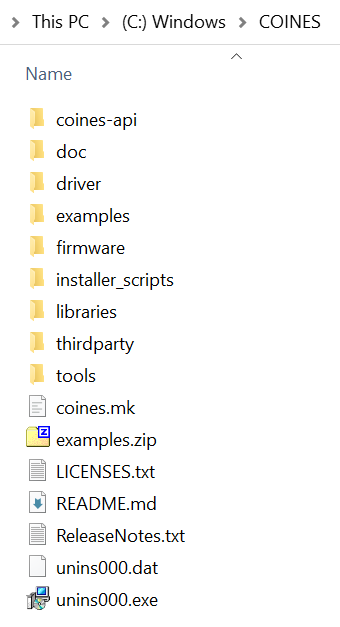
\includegraphics[width=0.4\textwidth]{coinesAPI_images/COINES_file_structure.png}
		\caption{COINES SDK file structure}
	\end{center}
\end{figure}
\bstlastpage

\end{document}
